\documentclass{article}



\usepackage{arxiv}

\usepackage[utf8]{inputenc} % allow utf-8 input
\usepackage[T1]{fontenc}    % use 8-bit T1 fonts
\usepackage{hyperref}       % hyperlinks
\usepackage{url}            % simple URL typesetting
\usepackage{booktabs}       % professional-quality tables
\usepackage{amsfonts}       % blackboard math symbols
\usepackage{nicefrac}       % compact symbols for 1/2, etc.
\usepackage{microtype}      % microtypography
\usepackage{lipsum}		% Can be removed after putting your text content
\usepackage{listings}
\usepackage{url}
\usepackage{graphicx}
\usepackage{longtable}

\lstset{
   basicstyle=\ttfamily\footnotesize
}

\title{MAST analysis of a Ravenscar precedence-constrained application with FPS and EDF scheduling}

%\date{September 9, 1985}	% Here you can change the date presented in the paper title
%\date{} 					% Or removing it

\author{
  Giovanni Jiayi Hu\\
  Department of Mathematics\\
  University of Padua, Italy I-35121\\
  \texttt{Email: giovannijiayi.hu@studenti.unipd.it} \\
  %% examples of more authors
   \And
   Alessio Gobbo \\
   Department of Mathematics\\
   University of Padua, Italy I-35121\\
   \texttt{Email: alessio.gobbo@studenti.unipd.it} \\
  %% \AND
  %% Coauthor \\
  %% Affiliation \\
  %% Address \\
  %% \texttt{email} \\
  %% \And
  %% Coauthor \\
  %% Affiliation \\
  %% Address \\
  %% \texttt{email} \\
  %% \And
  %% Coauthor \\
  %% Affiliation \\
  %% Address \\
  %% \texttt{email} \\
}

% Uncomment to remove the date
%\date{}

% Uncomment to override  the `A preprint' in the header
\renewcommand{\headeright}{}
\renewcommand{\undertitle}{Technical Report}

\begin{document}
\maketitle

\begin{abstract}
This paper describes a hard real-time application built with the Ravenscar profile of the Ada programming language and running on a real-time kernel of reduced size and complexity. The application is comprised of several tasks whose activation events present dependency relationships, and this characteristic allows interesting considerations during the different analysis we provide. We consider the same tasks under both Fixed-Priority Scheduling (FPS) and Earliest Deadline First (EDF) and evaluate different metrics like response times, jitters and blocking times. Throughout the sections, we also test the ability of the MAST analysis tools to describe a formal model of dependent tasks and to check their deadline satisfaction with less pessimism as possible without compromising correctness. Lastly, we offer some insight into the behaviour of both FPS and EDF systems under permanent and transient overload, a showcase of how classic real-time considerations may be revaluated to consider dependent tasks.
\end{abstract}


% keywords can be removed
% \keywords{First keyword \and Second keyword \and More}

\section{Introduction}

Embedded systems have to satisfy strict timing requirements and especially in the case of such hard real-time applications, predictability of the timing behaviour is an extremely important aspect. So it is the choice of a suitable design and development method, in conjunction with supporting tools that enable the real-time performance of a system to be analysed and simulated. The result can lead to a high level of confidence that the final system meets its real-time constraints.

As a matter of fact, the use of Ada has proven to be of great value within high integrity and real-time applications, thanks to language subsets of deterministic constructs which ensure full analysability of the code.  In embedded systems, the programmer is tied to become more concerned with the implementation and efficient manipulation of the abstract program entities representing the underlying hardware. Ada solves this issue by i.e. providing the programmer facilities for interrupt handling, access to shared variables and definition of task attributes.

Notably, the Ravenscar profile \cite{ycs} is a subset of the tasking model, restricted to meet the real-time community requirements for determinism, schedulability analysis and memory-boundedness, as well as being suitable for mapping to a small and efficient run-time system that supports task synchronization and communication.

Along with the Ravenscar profile, we have used a model for representing the temporal and logical elements of real-time applications, called MAST \cite{mast}. This model allows a very rich description of the system, including the effects of an event or message-based synchronization, multiprocessor and distributed architectures as well as shared resource synchronization.

The bare-board used throughout our analysis is the STM32F429I-Discovery, a low-cost and easy-to-use development kit to start with an STM32F4 microcontroller and equipped with an ARM Cortex-M4 core.
The board has been used along with the \texttt{ravenscar-full-stm32f429disco} runtime environment. The runtime implementation is provided by GNAT, a free-software compiler for the Ada language, and it is based upon the Open Ravenscar Real-Time Kernel \cite{ork}, which provides full conformance with the Ravenscar profile.

We have preferred the usage of a bare-board instead of the GNAT ARM emulator as we have noticed significant variance with the execution times measured on the latter. The board also includes a ST-LINK/V2 embedded debug tool, which can halt the processor, insert/remove breakpoints and execute instructions line by line \cite{debug-trace}.

We shall start the paper assuming Fixed Priority Scheduling (FPS), since its behaviour is more predictable and easier to reason about, and then introduce the Earliest Deadline First (EDF) scheduling by means of their differences.

The rest of the paper is organized as follows. The remaining Section 1 will provide an introduction to the fixed-priority scheduling and analysis, the application under consideration and some general notions of the Ada tasking model. A more formal description of our system is then presented in Section 2, followed by considerations about measuring the execution times and detecting deadline misses in Section 3 and 4, respectively. \\
Section 5 offers an in-depth description of the MAST model and its available analysis tools. Later, Sections 6 provides the insight of our FPS analysis with both stand-alone tasks and precedence relations, followed by a comparative EDF analysis in Section 7. Lastly, Section 8 includes some considerations of both systems under overload, whereas conclusions are contained in Section 8.

In the next sections, whenever we will use the term [RM], we will refer to a section of the Ada Language Reference Manual\footnote{\url{http://www.ada-auth.org/standards/rm12_w_tc1/html/RM-TOC.html}}.

\subsection{Fixed-priority scheduling and analysis}

In the fixed priority system under analysis, each task is assigned a static priority, and the schedule is generated based on the current priority value. According to the Rate Monotonic analysis \cite{rm-dm}, the fixed priorities are ordered based on the rates, so the task with the smallest period receives the highest priority. The rate (of job releases) of a task is the inverse of its period.

Another well-known fixed-priority algorithm is the Deadline Monotonic algorithm \cite{rm-dm}. This algorithm assigns priorities to tasks according to their relative deadlines: the shorter the relative deadline, the higher the priority.

Clearly, when the relative deadline of every task is proportional to its period, the two algorithms are identical. When the relative deadlines are arbitrary, the Deadline Monotonic algorithm performs better in the sense that it can sometimes produce a feasible schedule when the Rate Monotonic algorithm fails. In contrast, the RM algorithm always fails when the DM algorithm fails.

The schedulability analysis uses as inputs the given tasks of periods $T_i$ and execution times $C_i$  and checks one task $\tau_i$ at a time to determine whether the response times of all its jobs are equal to or less than its relative deadline $D_i$.

FPS analysis does not count on any relationship among the release times to hold, and identifies the worst-case combination of release times of any job  of task $\tau_i$, and all the jobs in the other tasks that have higher priorities. This combination is the worst because the response time of a job released under this condition is the largest possible for all combinations of release times.

This worst-case time instant is called the critical instant and corresponds to when the job is released at the same time with a job in every higher-priority task, e.g. all of the latter tasks are in phase. This is the case where the response time of the task is the largest and the analysis checks if it is still equal to or less than its relative deadline $D_i$.

To determine whether a task can meet all its deadlines, an analysis called time-demand analysis computes the total demand for processor time by a job released at a critical instant of the task and by all the higher-priority tasks as a function of time from the critical instant. It then checks whether this demand can be met before the deadline of the job.

To carry out the time-demand analysis on the taskset, we consider one task at a time, starting from the task $\tau_1$ with the highest priority in order of decreasing priority.
Assuming $t_0$ as the release time of the job from task $\tau_i$ at the critical instant, at time $t_0 + t$, for $t \ge 0$, the total (processor) time demand $w_i(t)$ of this job and all the higher-priority jobs released in $[t_0, t]$ is given by the following formula for $0 < t \le T_i$

$$
w_i(t) = C_i + \sum_{k=1}^{i-1} \lceil {t \over T_k} \rceil C_k
$$

If $w_i(t) > t$ for all $0 < t \le D_i$, this job cannot complete by its deadline. The task $\tau_i$, and hence the given system of tasks, cannot be feasibly scheduled by the fixed-priority algorithm.

Time-demand analysis can be usually depicted plotting the time-demand function as in Figure \ref{time-demand}.

\begin{figure}[!htbp]
\centering
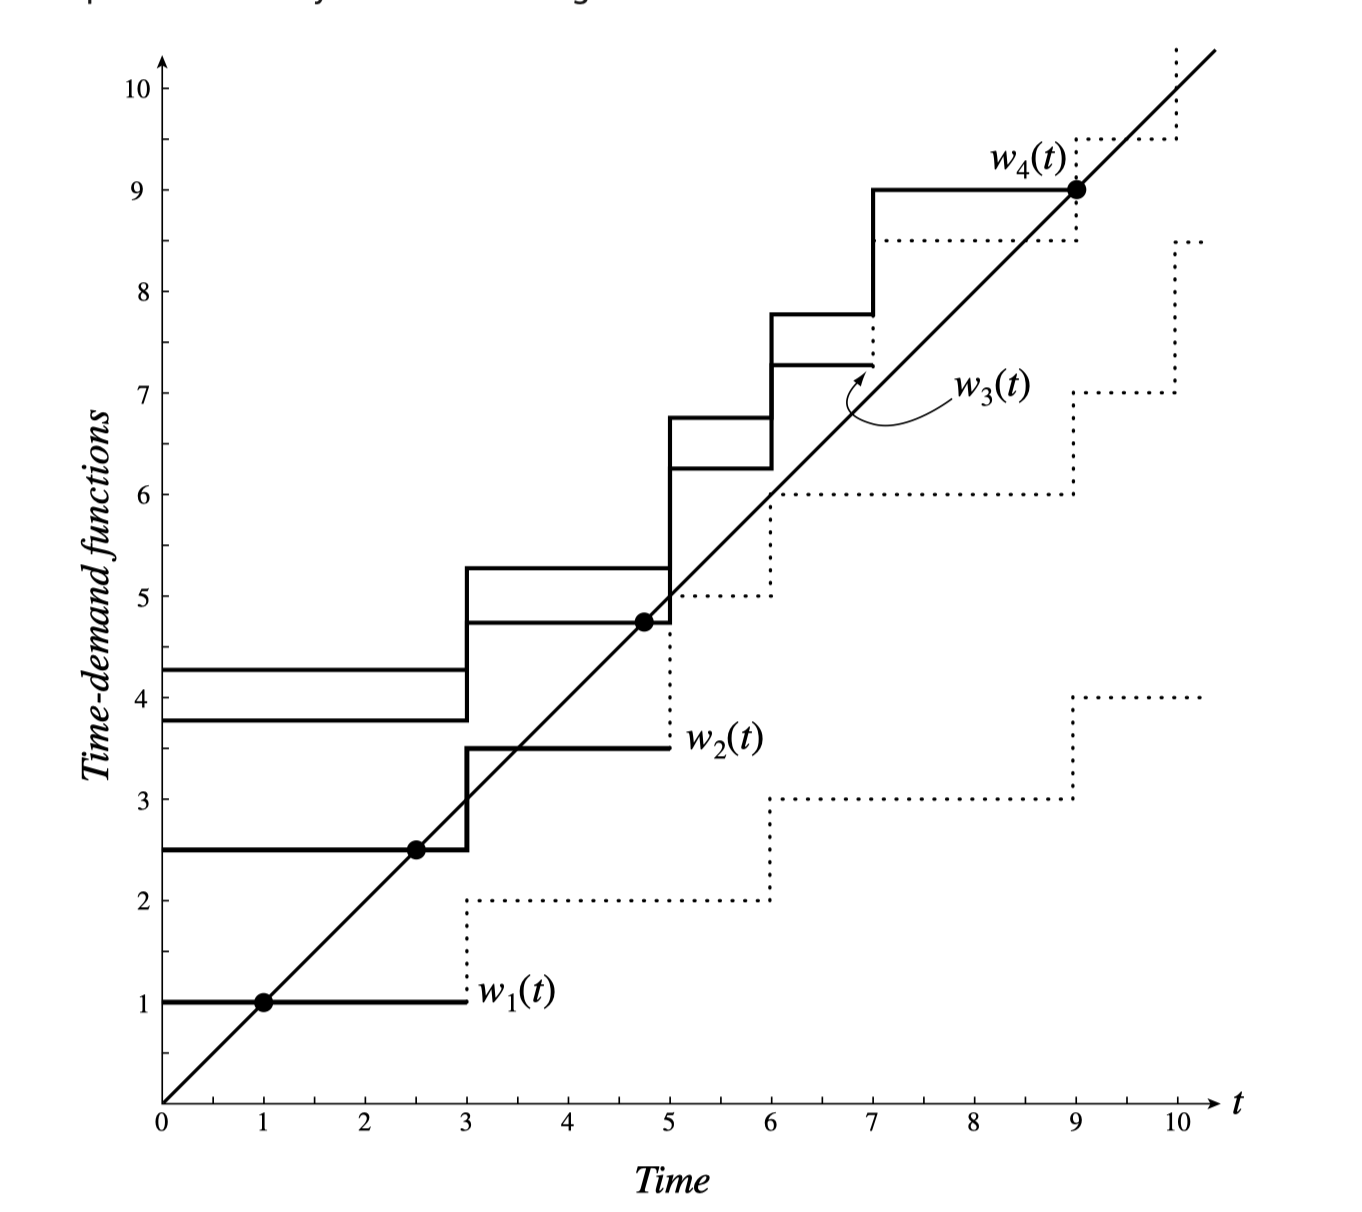
\includegraphics[width=4in]{images/time-demand}
\caption{Time-demand analysis example of four tasks $(T, C_i)$: (3,1), (5, 1.5), (7, 1.25), and (9, 0.5) \cite{rm-dm}}
\label{time-demand}
\end{figure}

\subsection{The application}\label{the-application}

\begin{figure}[!htbp]
\centering
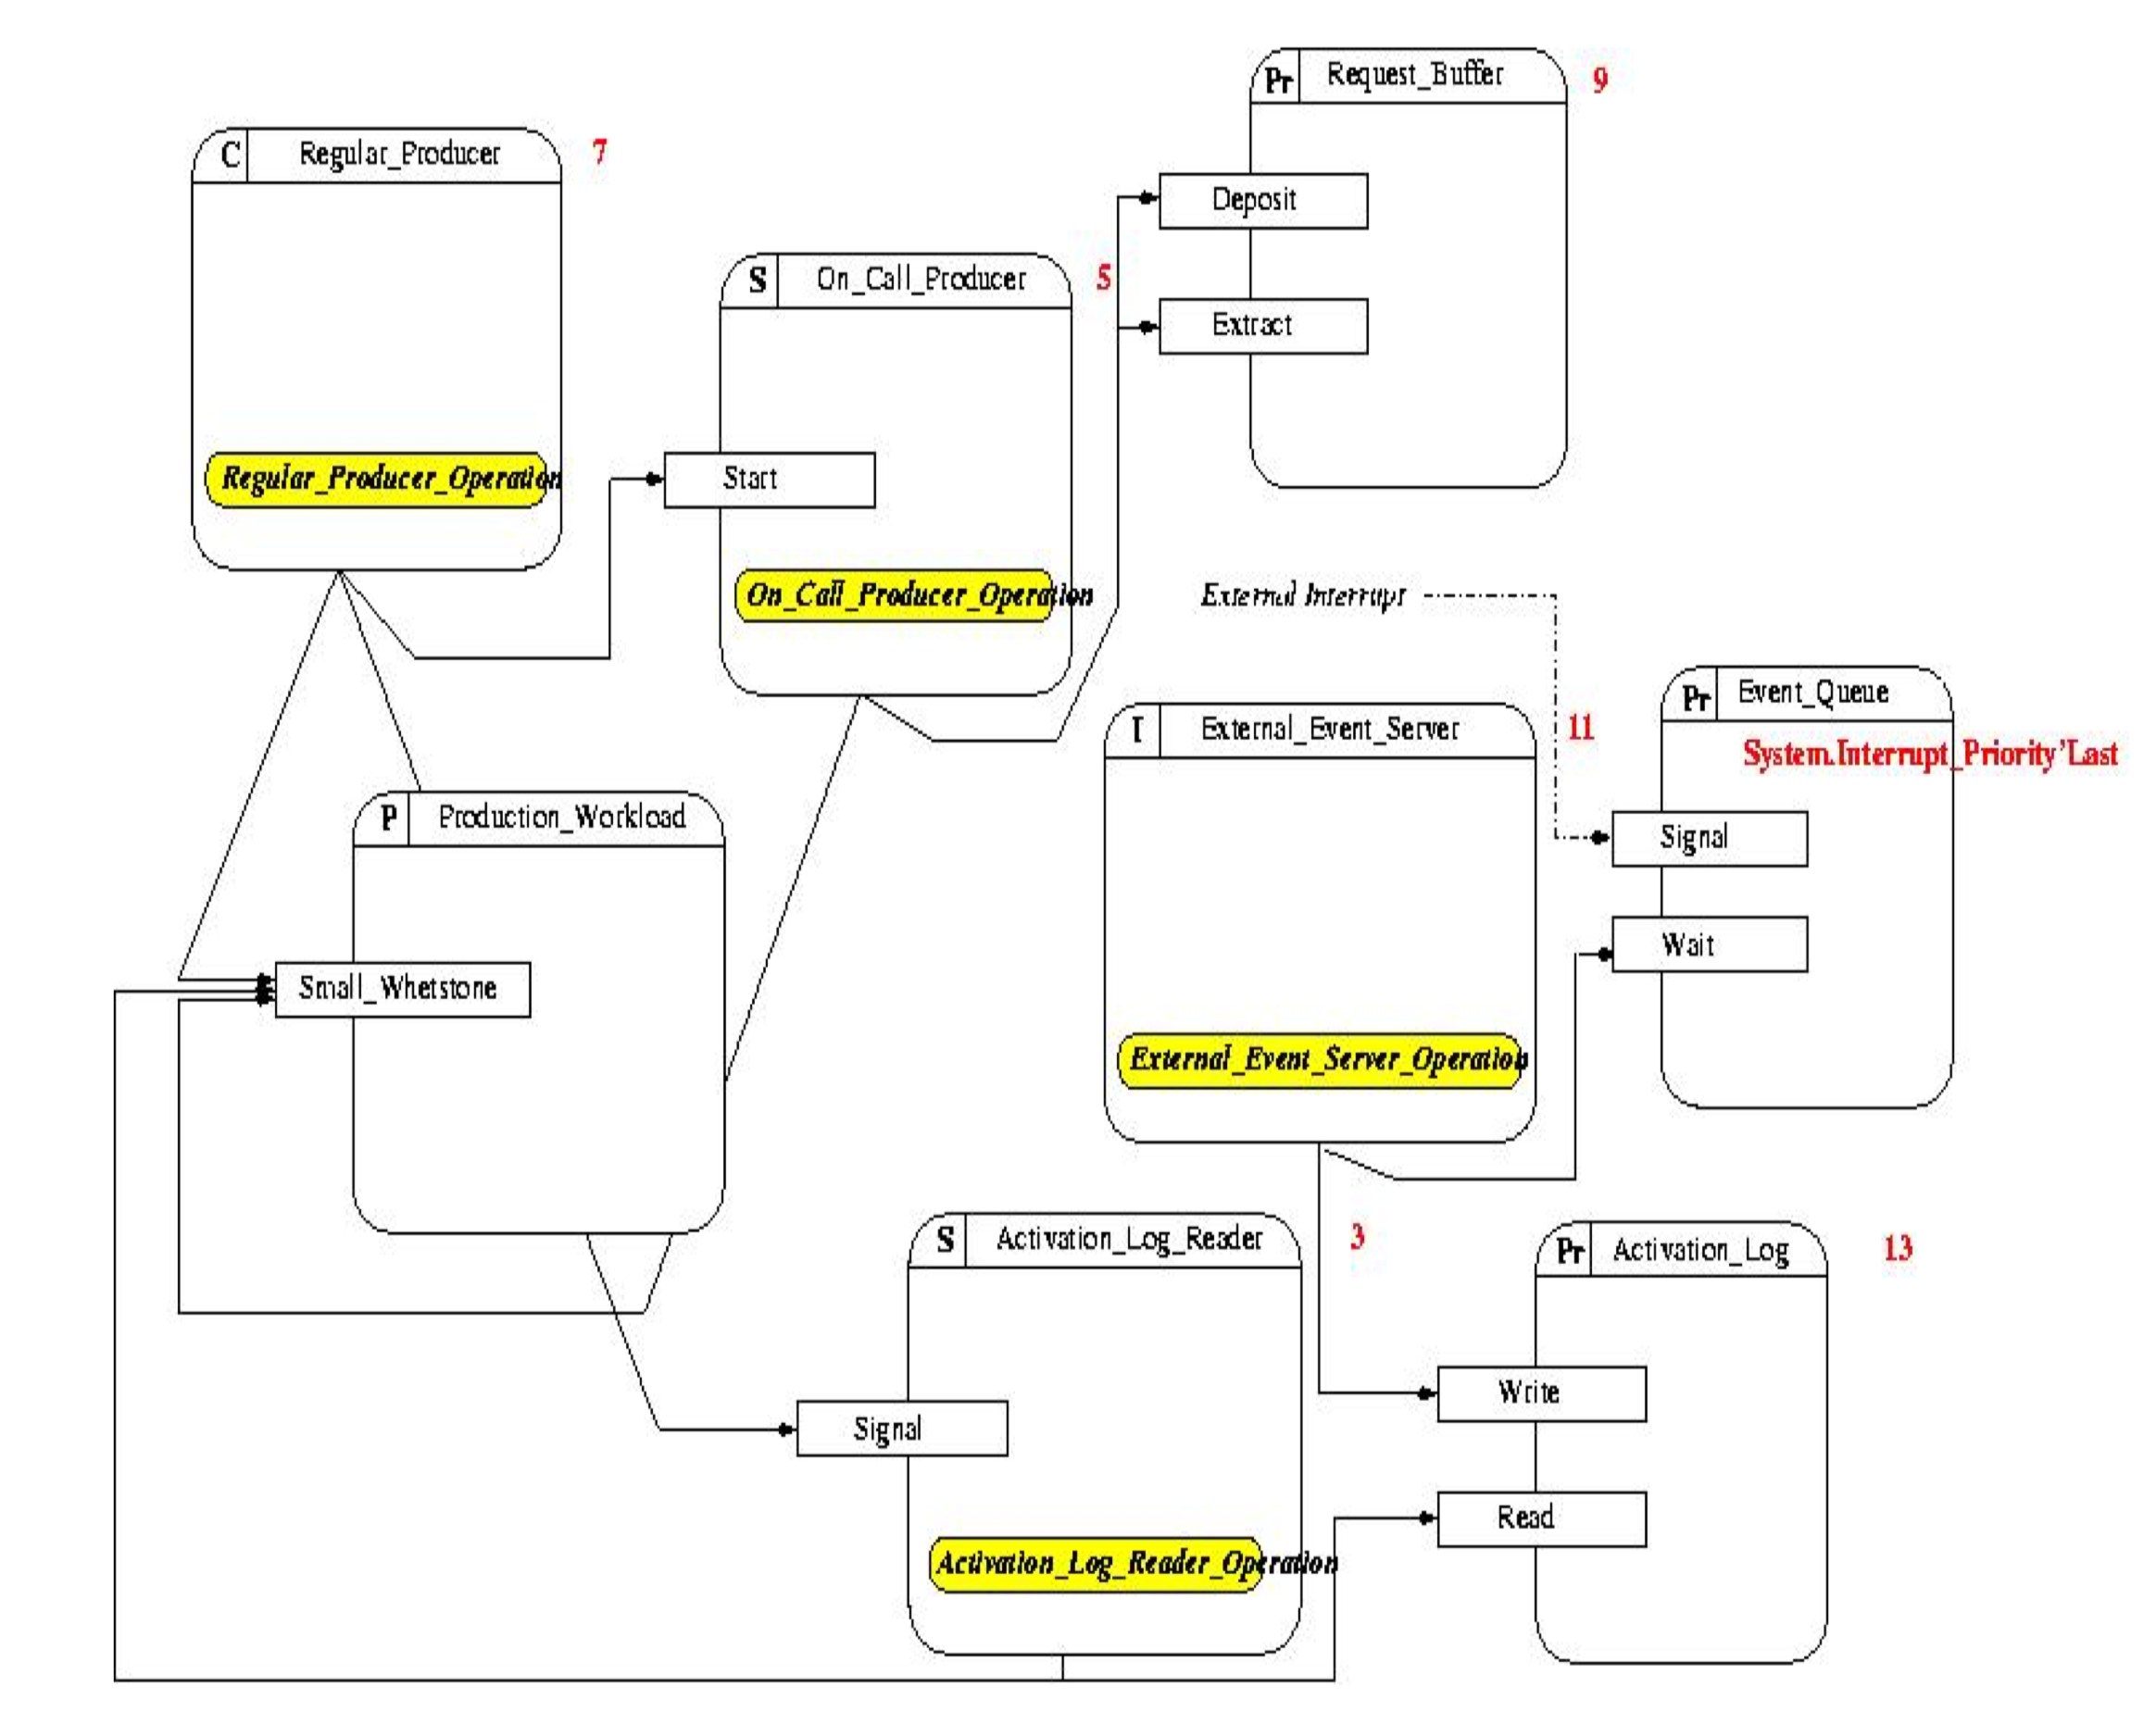
\includegraphics[width=5in]{images/ycs}
\caption{Architecture of the example application \cite{ycs}.}
\label{ycs}
\end{figure}

The example application presented in this paper is extracted from "Guide for the use of the
Ada Ravenscar Profile in
high integrity systems" \cite{ycs}. It includes a periodic process that handles orders for a variable amount of workload. Whenever the request level exceeds a certain threshold, the periodic process farms the excess loadout to a supporting sporadic process. While such orders are executed, the system may receive interrupt requests from an external manual push-button. Each interrupt treatment records an entry in an activation log.

When specific conditions hold, the periodic process releases a further sporadic process to perform a check on the interrupt activation entries recorded in the intervening period. The policy of work delegation adopted by the system allows the periodic process to ensure the constant discharge of a guaranteed level of workload.

The correct implementation of this policy also requires assigning the periodic process a higher priority than those assigned to the sporadic processes, so that guaranteed work can be performed in preference to subsidiary activities.

The application is comprised of the tasks and attributes in Table \ref{tab:tasks-attributes}. Static priorities are given based on the Deadline Monotonic scheduling \cite{rm-dm}, which is the most optimal between the fixed priority algorithms \cite{optimality-rm-dm}.

\begin{table}[!htbp]
   \centering
   \begin{tabular}{lllll}
     \toprule
     Task name & Task type & Period / Minimum inter-arrival time (ms) & Deadline (ms) & Priority  \\
     \midrule
     Regular\_Producer & Cyclic & 1000 & 500 & 7 \\
     On\_Call\_Producer & Sporadic & 3000 & 800 & 5 \\
     Activation\_Log\_Reader & Sporadic & 3000 & 1000 & 3 \\
     External\_Event\_Server & Interrupt sporadic & 5000 & 100 & 11 \\
     \bottomrule
   \end{tabular}
   \caption{Attributes of the tasks in the application \cite{ycs}}
   \label{tab:tasks-attributes}
\end{table}

Ada protected objects [RM 9.4] are used to ensure mutually exclusive access to shared resources, whereas protected entries are used only for task synchronization purposes where data exchange is involved.

In a real-time application, each protected object has a priority ceiling which represents the maximum priority of any task that calls the object. The Ada Real-Time Systems Annex supports the definition of  \texttt{Locking\_Policy} [RM D.3] and implements the resource locking protocol called Immediate Priority Ceiling Protocol (IPCP) \cite{ada-pcp}, which is similar to the Priority Ceiling Protocol (PCP).

PCP is an improvement of the Priority Inheritance Protocols (PIP) which allow a task to execute with an enhanced priority if it is blocking (or could block) a higher-priority task. In addition to PIP, PCP prevents deadlock and reduces blocking to its minimum value: every job is blocked at most once for the duration of a critical section, no matter how many jobs conflict with it \cite{pcp-blocking}.

The IPCP is similar to PCP in its use of the ceiling priority, but it has a different set of rules on how a task behaves under the ceiling locking protocol.

\begin{enumerate}
   \item A task may lock a protected object if it is not yet locked.
   \item When it enters a critical section, it immediately inherits the priority ceiling of the protected object and recovers its entry priority when it exits the section.
\end{enumerate}

This protocol effectively prevents any task from starting to execute until all the shared resources it needs are free. This means that no separate mutual exclusion mechanism, such as semaphores, is needed to lock shared resources. It is also cheap to implement at run time and incurs in fewer context switches. By raising priorities as soon as a resource is locked, whether a higher priority task is trying to access it or not, the protocol avoids the need to make complex scheduling decisions while tasks are already executing.

\begin{table}[!htbp]
   \centering
   \begin{tabular}{lll}
     \toprule
     Protected object names & User tasks & Ceiling priority  \\
     \midrule
     Request\_Buffer & Regular\_Producer (\texttt{Deposit}), On\_Call\_Producer (\texttt{Extract}) & 9 \\
     Event\_Queue & External interrupt (\texttt{Signal}), External\_Event\_Server (\texttt{Wait}) & System.Interrupt\_Priority'First \\
     Activation\_Log & External\_Event\_Server (\texttt{Write}), Activation\_Log\_Reader (\texttt{Read}) & 13 \\
     \bottomrule
   \end{tabular}
   \caption{Attributes of the protected objects in the application \cite{ycs}}
   \label{tab:po-attributes}
\end{table}

\subsection{Ada tasks for real-time systems}

In the Ada Ravenscar, a periodic task has an infinite loop within which there is a self-suspension statement that ensures that the task regularly executes \cite{ada-tasks}:

\begin{lstlisting}[language=Ada]
with Ada.Real_Time; use Ada.Real_Time;
...
task Periodic_Task;
   task body Periodic_Task is
      Period : Time_Span := Milliseconds(1000);
      -- define the period of the task, 1000 ms in this example
      Next : Time;
   begin
      Next := Clock;
      -- start time
      loop
         -- undertake the work of the task
         Next := Next + Period;
         delay until Next;
      end loop;
end Periodic_Task;
\end{lstlisting}

However, we should bear in mind that \texttt{Period} is the minimum length of time between the release times of instances of the task. The subsequent jobs will be released periodically only if the loop always completes within \texttt{Period} time units. If the response time of an instance of the thread exceeds the value, the next instance is released only as soon as the current instance completes. Therefore there will be both a deadline miss of the current job and a delay in activation of the subsequent instance.

A sporadic task requires a protected object instead to control its release:

\begin{lstlisting}[language=Ada]
task Sporadic_Task;
protected Sporadic_Controller is
   entry Wait_Next_Invocation;
   procedure Release_Sporadic;
private
   Barrier : Boolean := False;
end Sporadic_Controller;

task body Sporadic_Task is
begin
   loop
      Sporadic_Controller.Wait_Next_Invocation;
      -- undertake the work of the task
   end loop;
end Sporadic_Task;

protected body Sporadic_Controller is
   entry Wait_Next_Invocation when Barrier is
   begin
      Barrier := False;
   end;

   procedure Release_Sporadic is
   begin
      Barrier := True;
   end;
end Sporadic_Controller;
\end{lstlisting}

The task body for an event-triggered task that conforms to the Ravenscar Profile typically has, as its last statement, an outermost infinite loop whose first statement is either a call to a protected entry or a call to a Suspension Object \cite{ycs}. The Suspension Object is used when no other effect is required in the signalling operation; for example, no data is to be transferred from signaller to waiter. In contrast, the protected entry is used for more elaborate event signalling, when additional operations must accompany the resumption of the event-triggered task.

\subsection{Software interrupts}
As mentioned above, the system may receive interrupt requests (IR) from an external manual push-button. Such IR is handled by the NVIC Interrupt Controller, which is a part of the Cortex-M processor that handles the exceptions and the interrupt configurations, prioritization and masking \cite{arm}.

To automate the arrival of interrupts throughout our following analysis, we periodically trigger an IR via software by using a Software Trigger Interrupt Register (STIR). We first define a system package \texttt{ST.EXTI} where we gain access to the STM32F4 Interrupts and Events registers. Then, setting a pending bit to the appropriate interrupt line in the STIR triggers the IR for the external push-button.

Lastly, the whole process is executed within a new periodic task Force\_Interrupt, whose loop body simulates the worst-case sporadic behaviour of the interrupt. The worst-case happens when the subsequent interrupts arrive at the minimum interarrival time, used as period of the task.

\begin{lstlisting}[language=Ada]
with Ada.Real_Time; use Ada.Real_Time;
with Ada.Text_IO;
with ST; use ST;
with ST.EXTI; use ST.EXTI;

package body Force_Interrupt is
   Period : constant Ada.Real_Time.Time_Span :=
      Ada.Real_Time.Milliseconds (5000);
   Button_Line : constant Interrupt_Line := 0;
   --  The User Button is connected to EXTI0 (aka Line 0)

   task body Force_Interrupt is
      --  for periodic suspension
      Next_Time : Ada.Real_Time.Time;
   begin
      loop
         Next_Time := Next_Time + Period;

         EXTI.Software_Trigger_Interrupt_Register.Line :=
            (Button_Line => True, others => False);
         Ada.Text_IO.Put_Line ("Interrupt generated");

         delay until Next_Time; --  delay statement at end of loop
      end loop;
   end Force_Interrupt;
end Force_Interrupt;
\end{lstlisting}

The overhead introduced by the newly defined task is negligible and thus will not be considered during the different analysis of the paper.

\section{System model and notation}\label{model-notation}

The described application is a set of tasks executing in the same processor, grouped into entities called transactions \cite{tindell-offsets}. Each transaction $\Gamma_i$ is activated by a periodic sequence of external events with period $T_i$ , and contains a set of tasks. Each task is released when a relative time offset elapses after the arrival of the external event. Each activation of a task releases the execution of one instance of that task, called a \textit{job}.

\begin{figure}[!htbp]
\centering
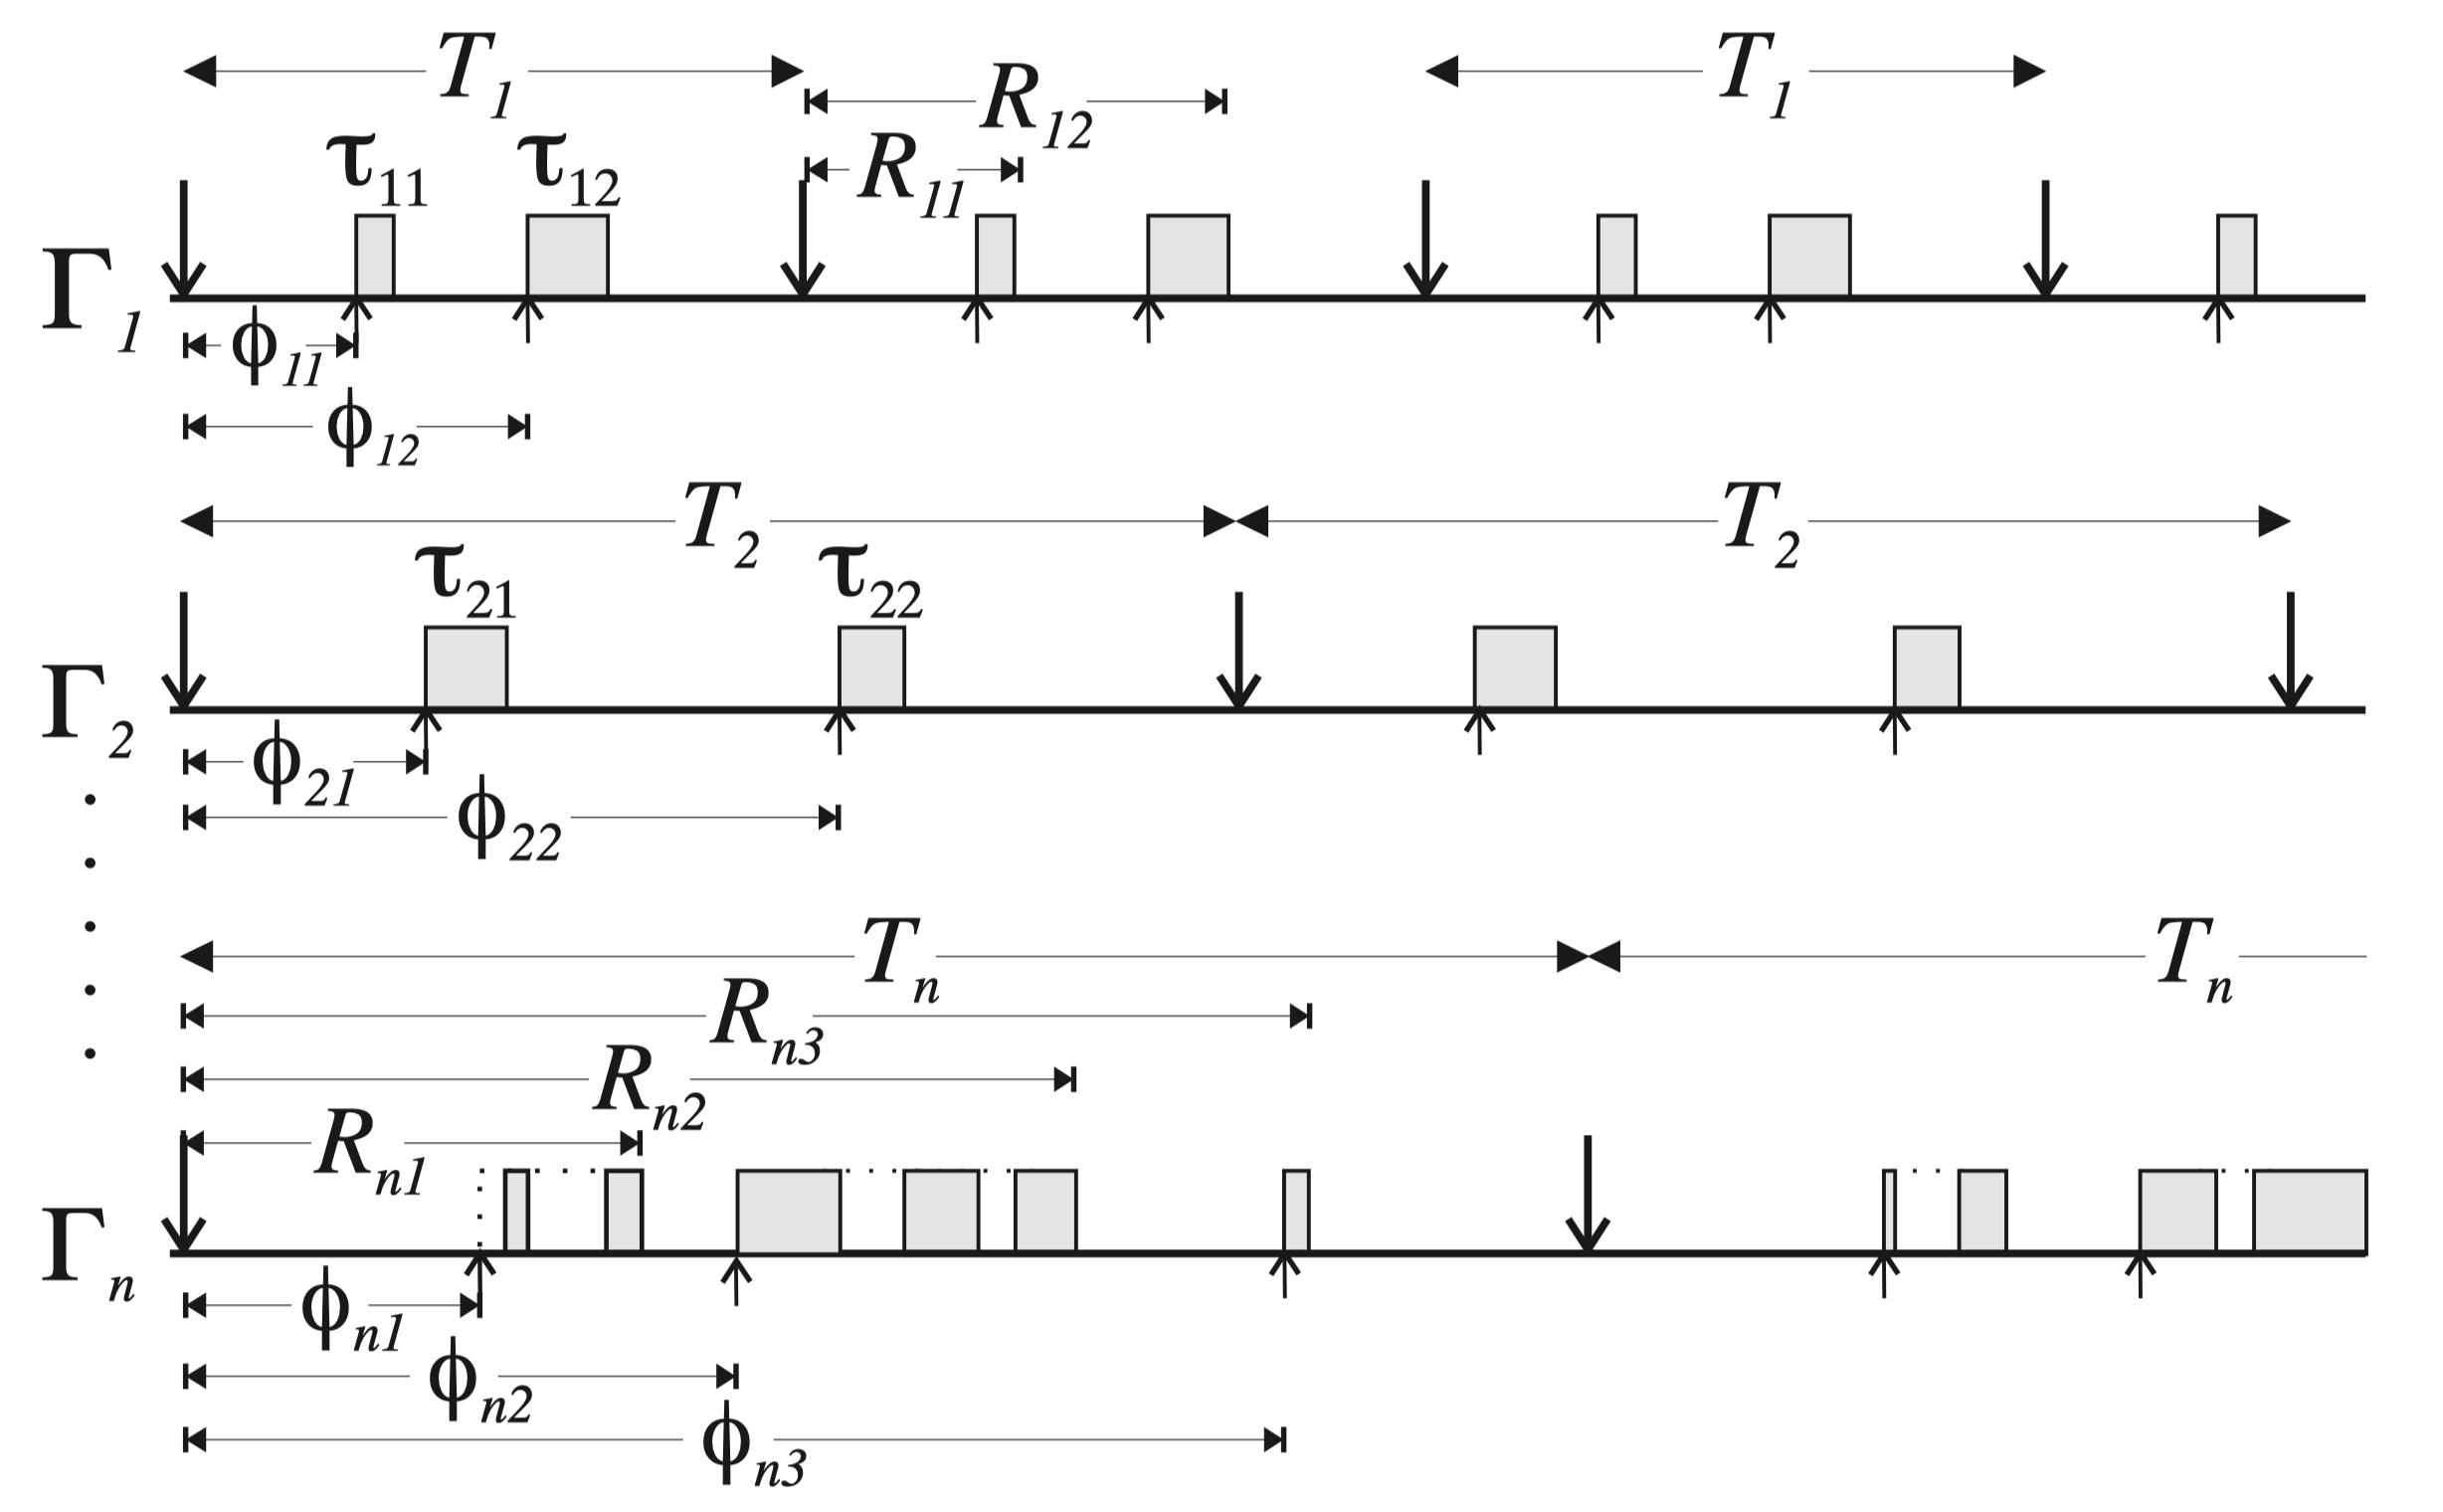
\includegraphics[width=5in]{images/transactions}
\caption{Timeline of a system composed of transactions with offsets \cite{pessimistic-rma}}
\label{transactions}
\end{figure}

Figure \ref{transactions} shows an example of such system: the horizontal axis represents time; down-pointing arrows represent the arrival of the external events associated to each transaction, while up-pointing arrows represent the activation times of each task; and shaded boxes represent task execution \cite{pessimistic-rma}. Each task has its own unique priority, and in this example, the task set is scheduled using a preemptive FPS.

Each task will be identified with two subscripts: the first one identifies the transaction to which it belongs, and the second one the position that the task occupies within the tasks of its transaction when they are ordered by increasing offsets. In this way, $\tau_{ij}$ will be the j-th task of transaction $\Gamma_i$, with an offset of $\Phi_{ij}$ and a worst-case execution time of $C_{ij}$. In addition, we will allow each task to have jitter, that is to have its activation time delayed by an arbitrary amount of time between 0 and the maximum jitter for that task, which we will call $J_{ij}$. This means that the activation time of task $\tau_{ij}$ may occur at any time between $t_0 + \Phi_{ij}$ and $t_0 + \Phi_{ij} + J_{ij}$, where $t_0$ is the instant at which the external event arrived.

The reason for this is that tasks must execute in order, i.e. On\_Call\_Producer can start executing only after the preceding task in the transaction, Regular\_Producer, has completed. The precedence constraints are modelled by assigning each task an initial offset and a maximum jitter \cite{tindell-offsets}. The initial offset $\Phi_{ij}$ of a periodic task is the instant of the first activation of the task. However, a task belonging to a transaction may start only after it has been activated, and the preceding task in the transaction has completed execution. Hence maximum jitter is the maximum time interval it can occur from the task activation until the completion time of the preceding task in the transaction.

In addition to maximum jitter, tasks offsets are allowed to vary dynamically, from one activation to the next, within a minimum and a maximum value: $\Phi_{ij} \in [\Phi_{ij\ min}, \Phi_{ij\ max}]$. Dynamic offsets are useful in systems in which tasks suspend themselves, like in the case of protected object entries. The task On\_Call\_Producer $\tau_{i2}$ calls the protected entry \texttt{Extract} and suspends itself until the task Regular\_Producer $\tau_{i1}$ replenishes the \texttt{Request\_Buffer}. The activation time of On\_Call\_Producer depends on the completion time of the Regular\_Producer, and thus the offset for task $\tau_{i2}$ is variable in the interval $\Phi_{i2} \in [R_{i1\ min}, R_{i1\ max}]$, where $R_{i1\ min}$ and $R_{i1\ max}$ are respectively the best-case and worst-case response times of task Regular\_Producer.

For each task $\tau_{ij}$ we define its response time as the difference between its completion time and the instant at which the task is released. The worst-case response time will be called $R_{ij}$. Each task has also an associated global deadline, $D_{ij}$, which is again relative to the arrival of the external event.

If tasks synchronize using shared resources in a mutually exclusive way, they will be using the aforementioned Immediate Priority Ceiling Protocol. The effects of lower priority tasks on a task under analysis $\tau_{ab}$ are bounded by an amount called the blocking term $B_{ab}$, calculated as the maximum of all the critical sections of lower priority tasks that have a priority ceiling higher than or equal to the priority of $\tau_{ab}$.

\subsection{Offset-based analysis}

Rate monotonic analysis (RMA) \cite{rm-dm} allows an approximate calculation of the worst-case response time of tasks in single-processor real time systems, including the effects of task synchronization, the presence of aperiodic tasks, the effects of deadlines before, at or after the periods of the tasks, tasks with varying priorities, overhead analysis, etc. However, classic RMA \cite{practitioner-common-data} cannot provide exact solutions in systems in which tasks with precedence relations. Classic techniques for these systems are based on the assumption that all tasks are independent, and thus they lead to pessimistic results \cite{pessimistic-rma}.

For building the worst-case scenario for a task $\tau_{ab}$ under analysis, the analysis must consider the critical instant that leads to the worst-case busy period. A task $\tau_{ab}$ busy period is an interval of time during which the CPU is busy processing task $\tau_{ab}$ or higher priority tasks. For tasks with offsets, it must take into account that the critical instant may not include the simultaneous arrival of all higher priority jobs, as it was the case when all tasks were independent. The existence of offsets makes it impossible for some sets of tasks to become active simultaneously.

Works on such problem have been the base of offset-based analysis, first proposed by Tindell and Clark \cite{tindell-offsets} and later improved by Palencia and Gonzàlez \cite{pessimistic-rma} who called it Worst-Case Analysis of Dynamic Offsets. In such analysis, the best and worst-case response times of each task are used to set the offset and the jitter of the successive task in the same transaction.

\section{Execution times}

To use the described model, upper bounds on the execution times are needed. Unfortunately, precise Worst-Case Execution Time (WCET) is hard to find due to pipelines, caches and other performance-enhancing techniques used on contemporary computer architectures \cite{wcet-problem}. These effects are reduced in the case of a more predictable bare-board environment, which can nevertheless suffer a small amount of indeterminism. Therefore pessimistic scheduling is needed in order to provide an offline guarantee that all hard deadlines will be met, but leads to poor processor utilisation.

\begin{figure}[!htbp]
\centering
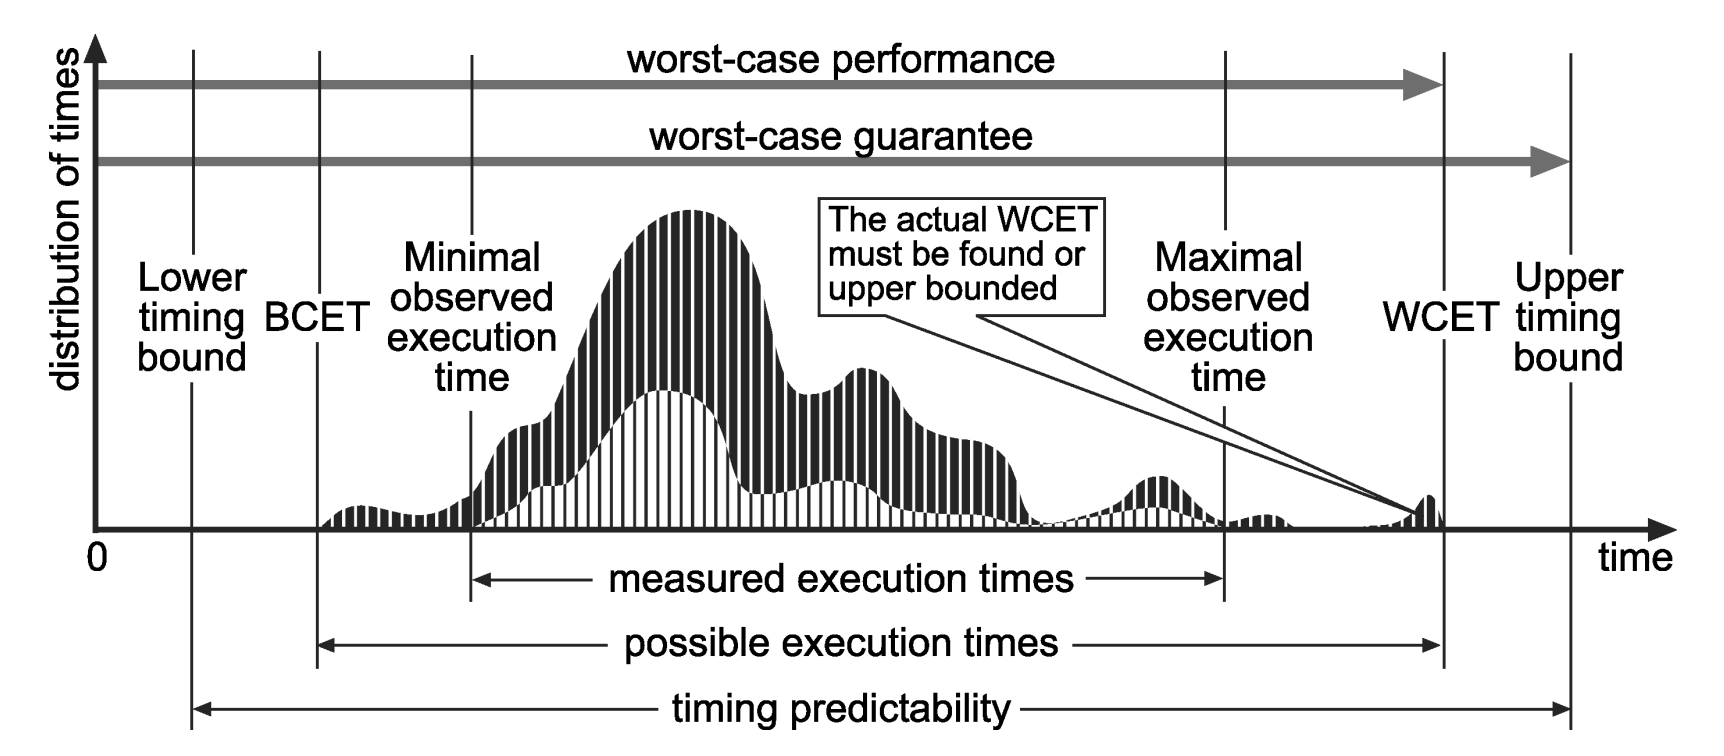
\includegraphics[width=5in]{images/wcet}
\caption{The lower curve represents a subset of measured executions. The darker curve, an envelope of the former, represents the times of all executions. \cite{wcet-problem}.}
\label{wcet-curve}
\end{figure}

Figure \ref{wcet-curve} shows the set of all execution times as the upper curve. Its minimum and maximum are the best- and worst-case execution times, respectively, abbreviated BCET and WCET. In most cases, the space is too large to exhaustively explore all possible executions and thereby determine the exact worst- and best-case execution times.

The conventional method to estimate execution time bounds is to measure the end-to-end execution time of the task for a subset of the possible executions. This determines the minimal observed and maximal observed execution times. These will, in general, overestimate the BCET and underestimate the WCET.

Nevertheless, we have adopted the same approach, aware of the mentioned perils. In most cases, we had deterministic execution times with always the same exact number of CPU cycles or with a difference less than 1$\mu$s, except for the Whetstone operations, which showed more significant variation. However, we always had shallow standard errors minor than 1\%. The example application is quite simple, comprised of few tasks with predictable executions and the only interrupts are the periodic ticker and the external push button.

Execution times are measured using two custom packages: \texttt{System\_Overhead} and \texttt{Task\_Metrics}. The former is able to provide the exact number of elapsed CPU ticks, which is then converted as seconds by dividing it with the clock frequency. It's used to measure runtime overhead, whereas the latter provides task execution time if self-suspension can happen, which would make usage of the clock ticks unsuitable.

\begin{lstlisting}[language=Ada]
-- system-overhead.ads
with System.BB.Time; use System.BB.Time;
with System.Semihosting;

package System_Overhead is
   pragma Preelaborate;

   procedure Start_Tracking;

   --  Avoid counting sub-program execution time
   procedure Start_Sub_Program;
   procedure End_Sub_Program;

   procedure End_Tracking (Item : String := "");

   procedure Log_Time;
   --  Just log the current clock time
end System_Overhead;

with System.BB.Time; use System.BB.Time;
with System.Semihosting;
\end{lstlisting}

\begin{lstlisting}[language=Ada]
-- system-overhead.adb
package body System_Overhead is
   Initial_Value : Time := 0;
   Start_Sub_Value : Time := 0;
   End_Sub_Value : Time := 0;

   procedure Start_Tracking is
   begin
      Initial_Value := Clock;
      Start_Sub_Value := 0;
      End_Sub_Value := 0;
   end Start_Tracking;

   procedure Start_Sub_Program is
   begin
      Start_Sub_Value := Clock;
   end Start_Sub_Program;

   procedure End_Sub_Program is
   begin
      End_Sub_Value := Clock;
   end End_Sub_Program;

   procedure End_Tracking (Item : String := "") is
      Now : constant Time := Clock;
      Sub_Program : Time;
      Elapsed : Time;
   begin
      -- Sometime End_Tracking may be called before Start_Tracking
      if Initial_Value = 0 then
         return;
      end if;

      Sub_Program := End_Sub_Value - Start_Sub_Value;
      Elapsed := Now - Initial_Value - Sub_Program;

      Put_Line (Item & Time'Image (Elapsed));
   end End_Tracking;

   procedure Log_Time is
   begin
      Put_Line (Time'Image (Clock));
   end Log_Time;

   procedure Put_Line (Item : String) is
   begin
      System.Semihosting.Put (Item & ASCII.CR & ASCII.LF);
   end Put_Line;
end System_Overhead;
\end{lstlisting}

The \texttt{System\_Overhead} package uses the board-specific \texttt{System.BB.Time} package, which provides the \texttt{Clock} function to read the real-time monotonic clock. It's the same primitive used under-the-hood by \texttt{Ada.Real\_Time} [RM D.8] to provide physical time as observed in the external environment.

The package \texttt{Task\_Metrics} has the same interface as \texttt{System\_Overhead}, but it replaces \texttt{System.BB.Time} with \texttt{Ada.Execution\_Time} [RM D.14] to measure the elapsed execution time of a task. The \texttt{ravenscar-full-stm32f429disco} runtime supports the Ada 2012 implementation to separately account for the execution time of interrupt handlers \cite{etc}.

The functionality of the real-time clock (RTC) and execution time clocks (ETCs) are quite similar: both clocks support high accuracy measurement of the monotonic passing of time since an epoch, and both support calling a protected handler when a given timeout time is reached. The main difference is that the RTC is always active, while an ETC is active only when its corresponding task or interrupt is executed.

\subsection{Semi-hosting}

It is worth mentioning the usage of semi-hosting \cite{semihosting}, which allows print messages to be transferred from the board to the host computer using the debug connection. Using semi-hosting for printing is usually much slower than UART because the semi-hosting mechanism needs to halt the processor, but on the other hand, the system tick timer \texttt{Sys\_Tick} counter is stopped during the transmission, thus avoiding affecting the schedule of the tasks. The example application has no timing requirements relative to external interrupts, with the exception of the manual push-button.

Both \texttt{System\_Overhead} and \texttt{Task\_Metrics} use semi-hosting to send execution time data to the host computer. Besides, it is leveraged also in the \texttt{ravenscar-full-stm32f429disco} runtime implementation of the \texttt{Ada.Text\_IO} package, whose method \texttt{Put\_Line} is called by the tasks.

The runtime defines a semi-hosting buffer size of 128 characters before flushing a string, therefore we have padded all the print messages with white space to reach the fixed size of 50 characters. By doing so, we have fixed execution time due to buffer insertion, simplifying MAST modelling of the \texttt{Put\_Line} operation.

\section{Deadline miss detection}

In later analysis, we will want to achieve the maximum schedulable utilisation by analyzing a MAST model with low utilisation and then increasing tasks utilisation until the system no longer meets its deadlines. However, for design attributes to turn into system properties, we must enforce them at runtime. In particular, we have to check that the jobs of the tasks always complete before their respective deadline, to ensure consistency between the MAST analysis and the execution \cite{timing-properties}.

Fortunately, Ada 2005 introduced a lower-level facility that maps a handler to a specific time without the need to use a separate task. The handler is associated with a timing event. When the event time is due and detected by the runtime, the handler code is executed.

The most effective way for an implementation to support timing events is to execute the handlers directly from the interrupt handler of the clock \cite{timing-events}, and this is indeed what happens in \texttt{ravenscar-full-stm32f429disco}.

\begin{lstlisting}[language=Ada]
-- deadline_miss.ads
with System;
with Ada.Real_Time; use Ada.Real_Time;
with Ada.Real_Time.Timing_Events; use Ada.Real_Time.Timing_Events;

package Deadline_Miss is
   type Deadline_Handler is limited private;

   procedure Set_Deadline_Handler (
      H: in out Deadline_Handler;
      Name : String;
      At_Time : in Time);
   procedure Cancel_Deadline_Handler (H: in out Deadline_Handler);

private
   protected type Deadline_Handler
     with Priority =>
       System.Interrupt_Priority'Last
   is
      procedure Notify_Deadline_Miss (Event : in out Timing_Event);

      procedure Set_Deadline_Handler (Name : String; At_Time : in Time);
      procedure Cancel_Deadline_Handler;

      private
         Tag : String(1..3) := "N/A";
         Event : Timing_Event;
   end Deadline_Handler;
end Deadline_Miss;
\end{lstlisting}

\begin{lstlisting}[language=Ada]
-- deadline_miss.adb
with Ada.Real_Time; use Ada.Real_Time;
with Ada.Text_IO; use Ada.Text_IO;

package body Deadline_Miss is
   protected body Deadline_Handler is
      procedure Notify_Deadline_Miss (Event : in out Timing_Event) is
      begin
         --raise Program_Error with "Detected deadline miss";
         Ada.Text_IO.Put_Line ("Deadline Miss Detected - " & Tag );
      end Notify_Deadline_Miss;

      procedure Set_Deadline_Handler (Name : String; At_Time : in Time) is
      begin
         Tag := Name;

         Set_Handler (Event, At_Time, Notify_Deadline_Miss'Access);
      end Set_Deadline_Handler;

      procedure Cancel_Deadline_Handler is
         Cancelled : Boolean;
         pragma Unreferenced (Cancelled);
      begin
         Cancel_Handler (Event, Cancelled);
      end Cancel_Deadline_Handler;
   end Deadline_Handler;

   procedure Set_Deadline_Handler (
      H: in out Deadline_Handler;
      Name : String;
      At_Time : in Time) is
   begin
      H.Set_Deadline_Handler (Name, At_Time);
   end Set_Deadline_Handler;

   procedure Cancel_Deadline_Handler (H : in out Deadline_Handler) is
   begin
      H.Cancel_Deadline_Handler;
   end Cancel_Deadline_Handler;
end Deadline_Miss;
\end{lstlisting}

The measured execution times include overrun detection overhead for Regular Producer, On Call Producer and Activation Log Reader.

\section{MAST}

MAST \cite{mast} is a Modeling and Analysis Suite for Real-Time Applications, and its main goal is to provide an open-source set of tools that enables engineers developing real-time applications to check the timing behaviour of their application, including schedulability analysis with hard timing requirements.

It is designed to handle both fixed priority and dynamic priority scheduled systems, although offset-based analysis for Earliest Deadline First scheduling is still missing as of the time of writing. However, within fixed priorities, different scheduling strategies are allowed, including preemptive and non-preemptive scheduling, interrupt service routines, sporadic server scheduling, and periodic polling servers.

The MAST model is designed to handle both single-processor as well as multiprocessor or distributed systems. In both cases, the emphasis is placed on describing event-driven systems in which each task may conditionally generate multiple events at its completion. A task may be activated by a conditional combination of one or more events. The external events arriving at the system can be of different kinds: periodic, unbounded aperiodic, sporadic, bursty, or singular (arriving only once).

The system model facilitates the independent description of overhead parameters such as processor overheads (including the overheads of the timing services). This frees us from the need to include all these overheads in the actual application model, thus simplifying it and eliminating much redundancy.

MAST provides also a graphical editor to generate the system using the MAST ASCII description. However, it's still immature to be reliable, and the presence of several graphical bugs causes an annoying experience. A graphical display of results is also available.

\subsection{The MAST Model}

We now proceed to describe the MAST model of the example application. In this phase, it will represent an FPS set of independent tasks, further sections will provide the needed changes to match a chain of dependant tasks or to support EDF scheduling. For a full reference to the MAST syntax, visit "Description of the MAST Model" \cite{mast-description}.

\subsubsection{Processing Resources}\label{processing-resources}

Processing Resources represent resources that are capable of executing abstract activities, including conventional CPU processors. Among its attributes, we have the range of priorities valid for normal operations on that processing resource and the speed factor. We have left the default value as speed factor, meaning that execution times will be expressed as seconds.

Normally when dealing with hard real-time analysis, we would also define only the Worst-Case Execution Time (WCET) of the operations but, since we have dynamic offsets depending on them, we include both best and worst execution times because we don't know for sure that always having the WCET corresponds to worst system performance. We may, for instance, have anomalies as in the case of multiple processors \cite{anomalies-multiprocessor}.

\begin{lstlisting}
Processing_Resource (
   Type                   => Regular_Processor,
   Name                   => cpu,
   Max_Interrupt_Priority => 255,
   Min_Interrupt_Priority => 241,
   Worst_ISR_Switch       => 2.578E-06,
   System_Timer           =>
      ( Type           => Ticker,
        Worst_Overhead => 3.844E-06,
        Period         => 0.001000),
   Speed_Factor           => 1.00);
\end{lstlisting}

The board is built with only one CPU, whereas the interrupt ranges are taken from the \texttt{System} package in the \texttt{ravenscar-full-stm32f429disco} runtime. Task priorities span from 1 to 240, while interrupt priorities go from 241 to 255. Thus it's possible to have at max 240 distinct task priorities if more priorities are needed, one can use the technique described in \cite{limited-priorities}.

The Interrupt Service Routine (ISR) overhead is measured as the time taken to run the \texttt{Interrupt\_Handler} in \texttt{System.BB.Board\_Support} package, without counting the execution time of the application interrupt handler. In Ada, the code in the handler itself executes at the hardware interrupt level. In contrast, the major part of the processing of the response to the interrupt is moved into an event response task, which executes at a software priority level with interrupts fully enabled.

The first procedure executes for a very short time-typically executing only the instructions that are strictly necessary to service the interrupt and reset the associated piece of hardware. The second one is implemented as a task that is activated from the interrupt handler and its priority is assigned as defined in Table \ref{tab:tasks-attributes}.

Both parts are not accounted into the ISR overhead. However, the overhead takes into account the management of the aforementioned Execution Time Clocks (ETC) \cite{etc}.

The system timer used by the board is Tick Scheduling \cite{tick-scheduling}, which represents a system that has a periodic clock interrupt that arrives at the system. When this interrupt arrives, all timed events whose expiration time has already passed, are activated.

Tick scheduling introduces two additional factors that must be accounted for in schedulability analysis. First, the fact that a job is ready may not be noticed and acted upon by the scheduler until the next clock interrupt. This introduces additional jitter that may delay the completion of the job.

Second, a self-suspended task is held in a queue which we will call the delay queue. When the scheduler executes, it scans the delay queue and moves the jobs that have been released since the last clock interrupt to the ready job queue and places them there in order of their priorities. Once in the ready queue, the jobs execute in priority order without intervention by the scheduler. The time the scheduler takes to scan and move the jobs introduces additional scheduling overhead. Similar overhead must be accounted for any timing events that need to be triggered.

The scheduling overhead is accounted for in the analysis using the technique described in \cite{effects-runtime}. MAST can model the scheduler as a periodic task $\tau_0$ whose period is $p_0$. This task has the highest priority among all tasks in the system. Its execution time $C_0$ is the amount of time the scheduler takes to service the clock interrupt. This time is spent even when there is no job in the pending job queue.

In the \texttt{ravenscar-full-stm32f429disco} runtime, the period $p_0$ of the tick is 1ms, defined in the \texttt{System.BB.Board\_Support} package and the worst overhead is measured as the time taken to execute \texttt{Timer\_Interrupt\_Handler}, the trap handler defined in the same package for the \texttt{Sys\_Tick} trap.

\subsubsection{Schedulers}

Schedulers represent the runtime procedures that implement the appropriate scheduling strategies to manage the amount of CPU processing capacity. They can have a hierarchical structure to model hierarchical scheduling \cite{hierarchical-scheduling}, but the example application has only one primary scheduler with fixed priority policy.

\begin{figure}[!htbp]
\centering
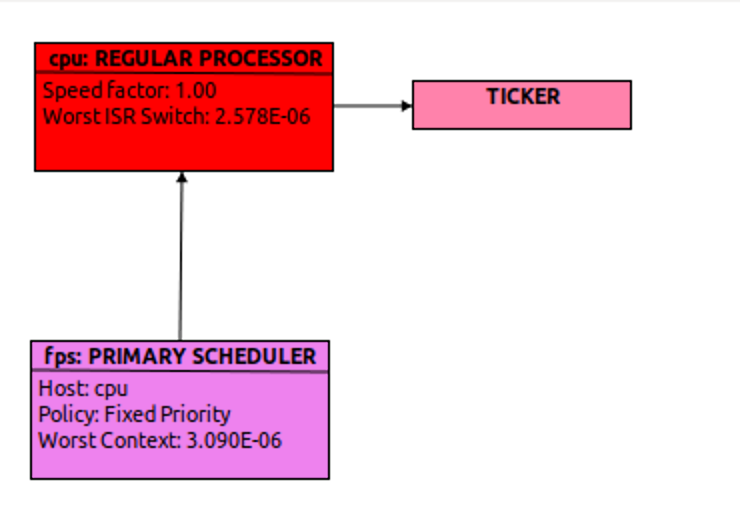
\includegraphics[width=3in]{images/primary-scheduler}
\caption{Fixed Priority Scheduler which manages the CPU}
\label{primary-scheduler}
\end{figure}

\begin{lstlisting}
Scheduler (
   Type            => Primary_Scheduler,
   Name            => fps,
   Host            => cpu,
   Policy          =>
      ( Type                 => Fixed_Priority,
        Worst_Context_Switch => 3.090E-06,
        Max_Priority         => 240,
        Min_Priority         => 1));
\end{lstlisting}

The context switch overhead is measured as time to set the context switch interrupt \texttt{Pend\_SV} as pending and the execution time of \texttt{Pend\_SV\_Handler} in the \texttt{System.BB.CPU\_Primitives.Context\_Switch\_Trigger} package, which saves the registers of active context and restores the ones of the new context. One some platforms, like in the case of the STM32F429I-Discovery board equipped with an ARM Cortex-M4 core, the context switch requires the triggering of a trap \cite{pendsv}. Then context switching is usually carried out in the \texttt{Pend\_SV} trap handler.

\subsubsection{Scheduling Servers}

Scheduling Servers represent schedulable entities in a processing resource, in particular, if the resource is a processor, the scheduling server is a task or thread of control. As a matter of fact, each of them has a priority and a type, which for our application may be \texttt{Fixed\_Regular\_Policy} or \texttt{Interrupt\_FP\_Policy}. The former represents a regular preemptive fixed priority, whereas the latter models an interrupt service routine. In reality, we have not used a \texttt{Interrupt\_FP\_Policy} as the interrupt overhead is negligible.

\begin{figure}[!htbp]
\centering
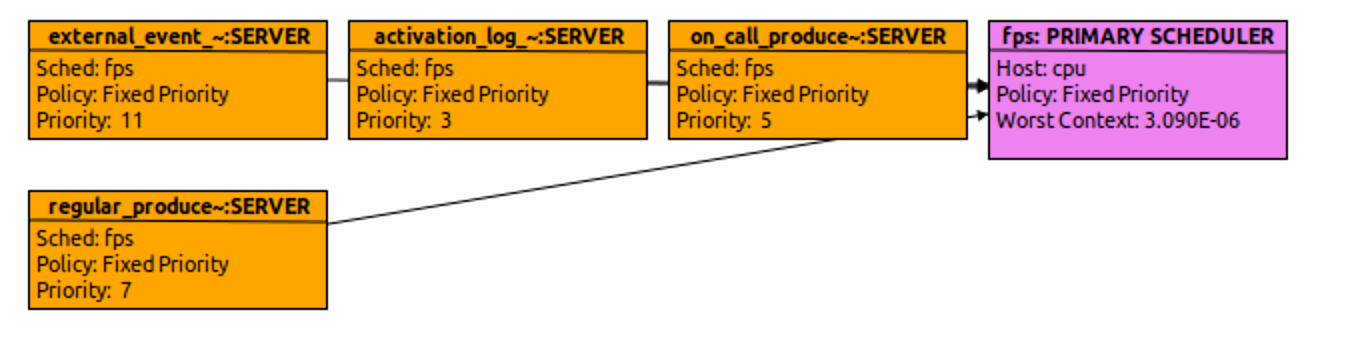
\includegraphics[width=5in]{images/scheduling-servers}
\caption{Scheduling Servers representing the application tasks}
\label{scheduling-servers}
\end{figure}

\begin{lstlisting}
Scheduling_Server (
   Type                       => Regular,
   Name                       => regular_producer,
   Server_Sched_Parameters    =>
      ( Type         => Fixed_Priority_Policy,
        The_Priority => 7,
        Preassigned  => YES),
   Scheduler                  => fps);

Scheduling_Server (
   Type                       => Regular,
   Name                       => on_call_producer,
   Server_Sched_Parameters    =>
      ( Type         => Fixed_Priority_Policy,
        The_Priority => 5,
        Preassigned  => YES),
   Scheduler                  => fps);

Scheduling_Server (
   Type                       => Regular,
   Name                       => activation_log_reader,
   Server_Sched_Parameters    =>
      ( Type         => Fixed_Priority_Policy,
        The_Priority => 3,
        Preassigned  => YES),
   Scheduler                  => fps);

Scheduling_Server (
   Type                       => Regular,
   Name                       => external_event_server,
   Server_Sched_Parameters    =>
      ( Type         => Fixed_Priority_Policy,
        The_Priority => 11,
        Preassigned  => YES),
   Scheduler                  => fps);
\end{lstlisting}

\subsubsection{Shared Resources}

Shared Resources represent resources that are shared among different tasks, and that must be used in a mutually exclusive way. Therefore, protected objects are modelled as Shared Resourses that use the Immediate Priority Ceiling Protocol described above.

\begin{figure}[!htbp]
\centering
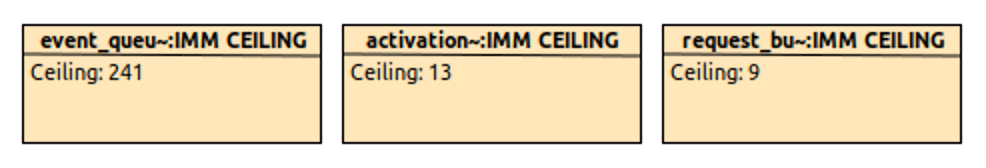
\includegraphics[width=4in]{images/shared-resources}
\caption{Shared Resources of the application}
\label{shared-resources}
\end{figure}

\begin{lstlisting}
Shared_Resource (
   Type        => Immediate_Ceiling_Resource,
   Name        => request_buffer,
   Ceiling     => 9,
   Preassigned => YES);

Shared_Resource (
   Type        => Immediate_Ceiling_Resource,
   Name        => activation_log,
   Ceiling     => 13,
   Preassigned => YES);

Shared_Resource (
   Type        => Immediate_Ceiling_Resource,
   Name        => event_queue,
   Ceiling     => 241,
   Preassigned => YES);
\end{lstlisting}

\subsubsection{Operations}

MAST Operations represent a piece of code to be executed by the processor. We have used the following classes of operations:

\begin{itemize}
   \item \textbf{Simple}: it represents a simple piece of code or a message. It may have the list of shared resources to lock before executing the operation, and the list of shared resources that must be unlocked after executing the operation. Simple Operations have been used to model methods of protected objects. The execution time is measured from the first line of the method to the last one, thus it doesn't include the runtime overhead associated with invoking protected methods.
   \item \textbf{Composite}: it represents an operation composed of an ordered sequence of other operations, simple or composite. The execution time attribute of this class cannot be set because it is the sum of the execution times of the comprised operations.
   \item \textbf{Enclosing}: it represents an operation that contains other operations as part of its execution, but in this case the total execution time must be set explicitly; it is not the sum of execution times of the comprised operations, because other pieces of code may be executed in addition. For each protected method, there is an Enclosing Operation which takes into account the overhead associated with calling protected methods. Sometimes it corresponds to a method defined by the application, other times it's defined in the model specifically to include the runtime overhead. By doing so, we can define the caller procedures as simple Composite operations.
\end{itemize}

Examples of protected methods as Simple Operations:

\begin{lstlisting}
Operation (
   Type                       => Simple,
   Name                       => rb_deposit,
   Worst_Case_Execution_Time  => 2.000E-06,
   Shared_Resources_To_Lock   =>
      ( request_buffer),
   Shared_Resources_To_Unlock =>
      ( request_buffer));

Operation (
   Type                       => Simple,
   Name                       => rb_extract,
   Worst_Case_Execution_Time  => 2.000E-06,
   Shared_Resources_To_Lock   =>
      ( request_buffer),
   Shared_Resources_To_Unlock =>
      ( request_buffer));
\end{lstlisting}

Examples of Enclosing Operations including protected methods overhead:

\begin{lstlisting}
Operation (
   Type                     => Enclosing,
   Name                     => ocp_start,
   Worst_Case_Execution_Time=> 6.000E-06,
   Composite_Operation_List =>
      ( rb_deposit));

Operation (
   Type                     => Enclosing,
   Name                     => rb_extract_enclosing,
   Worst_Case_Execution_Time=> 7.000E-06,
   Composite_Operation_List =>
      ( rb_extract));
\end{lstlisting}

A complete example of the MAST representation of a job of the task Regular\_Producer:

\begin{lstlisting}
Operation (
   Type                       => Simple,
   Name                       => rp_small_whetstone,
   Worst_Case_Execution_Time  => 0.019363);

Operation (
   Type                       => Simple,
   Name                       => due_activation,
   Worst_Case_Execution_Time  => 1.000E-06);

Operation (
   Type                     => Enclosing,
   Name                     => ocp_start,
   Worst_Case_Execution_Time=> 6.000E-06,
   Composite_Operation_List =>
      ( rb_deposit));

Operation (
   Type                       => Simple,
   Name                       => check_due,
   Worst_Case_Execution_Time  => 1.000E-06);

Operation (
   Type                       => Simple,
   Name                       => alr_signal,
   Worst_Case_Execution_Time  => 5.000E-06);

Operation (
   Type                       => Simple,
   Name                       => put_line,
   Worst_Case_Execution_Time  => 1.400E-05);

Operation (
   Type                     => Composite,
   Name                     => rp_operation,
   Composite_Operation_List =>
      ( rp_small_whetstone,
        due_activation,
        ocp_start,
        check_due,
        alr_signal,
        put_line));

Operation (
   Type                     => Composite,
   Name                     => regular_producer,
   Composite_Operation_List =>
      ( overrun_detection,
        rp_operation,
        delay_until));
\end{lstlisting}

The Small\_Whetstone algorithm allows controlling the computational workload of Regular\_Producer, On\_Call\_Producer and Activation\_Log\_Reader. By changing the workload parameters of \texttt{Small\_Whetstone} in the application, we will be able to test different utilisation of the system with likewise ease in updating the MAST model.

The Whetstone execution time is proportional to the workload parameter and exhibits deterministic behaviour. If we wanted to try what would happen by increasing the load of factor 10, we would just multiply the WCET in the model by 11, without the need to measure all the Enclosing operations again, since all the methods which use Whetstone are defined as Composite. However, we have been careful to avoid forgetting to include any overhead in an Enclosing method, and we have made sure they are not impacted by any change of the Whetstone workload.

\subsubsection{Transactions}

A Transaction represents a transaction of our model (see Section \ref{model-notation}) as a graph of event handlers and events, and form interrelated activities executed in the system. A Transaction is defined with three different components: a list of External Events, a list of Internal Events (with their timing requirements if any), and a list of Event Handlers.

Events may be internal or external and represent channels of event streams, through which individual event instances may be generated.

Internal Events are generated by an Event Handler. Internal Events have timing requirements, a Global Deadline relative to the arrival of a Referenced External Event. The MAST language also allows using Local Deadlines, relative to the arrival of the event that activated that Event Handler. All of our deadlines are Hard Deadlines, e.g. they must be met in all cases, including the worst case.

External events model the interactions of the system with external components or devices through interrupts, signals, etc., or with hardware timing devices. They have a double role in the model: on the one hand, they establish the rates or arrival patterns of activities in the system. On the other hand, they provide references for defining global timing requirements. MAST supports different arrival patterns, of which we used the following: \textit{Periodic} represents a stream of events that are generated periodically, such as from the Tick Scheduling; \textit{Sporadic} as a stream of aperiodic events that have a minimum interarrival time.

\begin{figure}[!htbp]
\centering
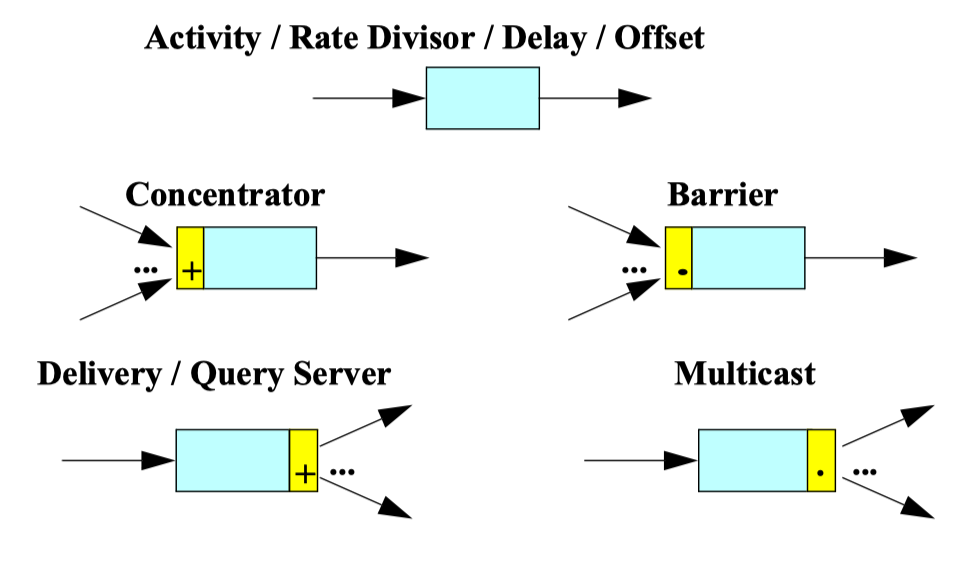
\includegraphics[width=3in]{images/event-handlers}
\caption{Event Handlers}
\label{event-handlers}
\end{figure}

Event Handlers in figure \ref{event-handlers} represent actions that are activated by the arrival of one event, and that in turn generate one or more events at their output. There are two fundamental classes of Event Handlers. The Activities represent the execution of an operation by a Scheduling Server (a task), in a processing resource (the CPU). The other kinds of Event Handlers are just a mechanism for handling events, with no runtime effects. In the model, we have used the following classes:

\begin{itemize}
   \item \textit{Activity}: an instance of an operation to be executed by a Scheduling Server;
   \item \textit{System Timed Activity}: an activity that is activated by the system timer, and thus is subject to the aforementioned jitter associated with it;
   \item \textit{Multicast}: it is an event handler that generates one event in every one of its outputs each time an input event arrives;
   \item \textit{Rate Divisor}: it is an event handler that generates one output event when a number of input events equal to the Rate Factor have arrived;
   \item \textit{Offset}: an event handler that generates its output event after a time interval has elapsed from the arrival of some (previous) external event. If the time interval has already passed when the input event arrives, the output event is generated immediately.
\end{itemize}

We now proceed to model the three transactions which model the respective independent tasks. We will start with an initial analysis of the system as stand-alone tasks, then compare its maximum utilisation with the model using dynamic offsets to represent dependant tasks.

\begin{figure}[!htbp]
\centering
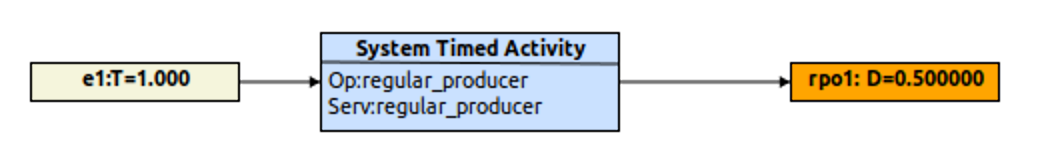
\includegraphics[width=5in]{images/transaction-rp}
\caption{Regular\_Producer transaction}
\label{transaction-rp}
\end{figure}

\begin{lstlisting}
Transaction (
   Type            => regular,
   Name            => rp_transaction,
   External_Events =>
      ( ( Type       => Periodic,
          Name       => e1,
          Period     => 1.000,
          Max_Jitter => 0.000,
          Phase      => 0.000)),
   Internal_Events =>
      ( ( Type => Regular,
          Name => rpo1,
          Timing_Requirements =>
            ( Type             => Hard_Global_Deadline,
              Deadline         => 0.500000,
              Referenced_Event => e1))),
   Event_Handlers  =>
      ( (Type               => System_Timed_Activity,
         Input_Event        => e1,
         Output_Event       => rpo1,
         Activity_Operation => regular_producer,
         Activity_Server    => regular_producer)));
\end{lstlisting}

The main event stream is modelled as a transaction activated by the periodic system timer, with a period of 1s. The event is handled by the \texttt{regular\_producer} operation, representing a job of the same name. The Event Handler is of type \texttt{System\_Timed\_Activity} to take into account the jitter caused by the tick scheduling.

\begin{figure}[!htbp]
\centering
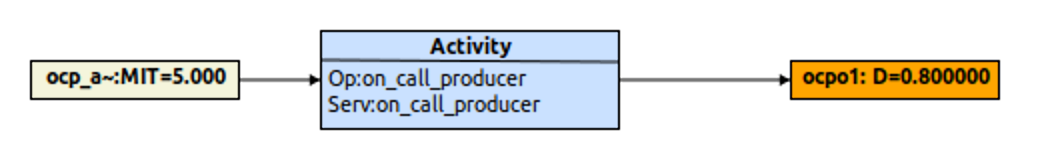
\includegraphics[width=5in]{images/transaction-ocp}
\caption{On\_Call\_Producer transaction}
\label{transaction-ocp}
\end{figure}

\begin{figure}[!htbp]
\centering
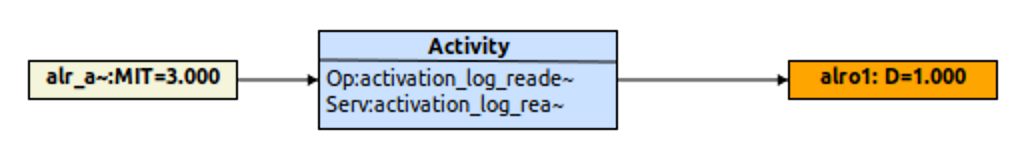
\includegraphics[width=5in]{images/transaction-alr}
\caption{Activation\_Log\_Reader transaction}
\label{transaction-alr}
\end{figure}

\begin{lstlisting}
Transaction (
   Type            => regular,
   Name            => ocp_transaction,
   External_Events =>
      ( ( Type             => Sporadic,
          Name             => ocp_activation,
          Min_Interarrival => 3.000)),
   Internal_Events =>
      ( ( Type => Regular,
          Name => ocpo1,
          Timing_Requirements =>
            ( Type             => Hard_Global_Deadline,
              Deadline         => 0.800000,
              Referenced_Event => ocp_activation))),
   Event_Handlers  =>
      ( (Type               => Activity,
         Input_Event        => ocp_activation,
         Output_Event       => ocpo1,
         Activity_Operation => on_call_producer,
         Activity_Server    => on_call_producer)));
\end{lstlisting}

The sporadic On\_Call\_Producer event stream is modelled as activated by a bounded aperiodic event, with a minimum interarrival time of 3s. Similar modelling has been done for the Activation\_Log\_Reader sporadic task.

\begin{figure}[!htbp]
\centering
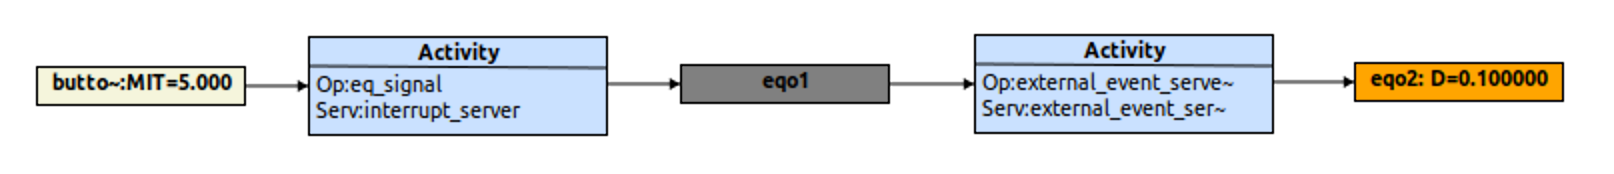
\includegraphics[width=5in]{images/transaction-eq}
\caption{External push-button transaction}
\label{transaction-eq}
\end{figure}

\begin{lstlisting}
Transaction (
   Type            => regular,
   Name            => interrupt_transaction,
   External_Events =>
      ( ( Type             => Sporadic,
          Name             => button_click,
          Avg_Interarrival => 0.000,
          Distribution     => UNIFORM,
          Min_Interarrival => 5.000)),
   Internal_Events =>
      ( ( Type => Regular,
          Name => eqo1,
          Timing_Requirements =>
            ( Type             => Hard_Global_Deadline,
              Deadline         => 0.100000,
              Referenced_Event => button_click))),
   Event_Handlers  =>
      ( (Type               => Activity,
         Input_Event        => button_click,
         Output_Event       => eqo1,
         Activity_Operation => external_event_server,
         Activity_Server    => external_event_server)));
\end{lstlisting}

The push-button interrupt event stream is modelled as triggered by a sporadic event of 5s as minimum interarrival time and it's handled by the \texttt{external\_event\_server} job at software priority. The interrupt handler at hardware interrupt priority has not been modelled since it's execution time is negligible.

\subsection{MAST analysis}\label{mast-analysis}

As of the time of writing, MAST is at version 1.5.1 and supports the analysis tools \cite{mast-analysis} in Figure \ref{mast-analysis-tools}. The techniques relevant for this paper are:

\begin{figure}[!htbp]
\centering
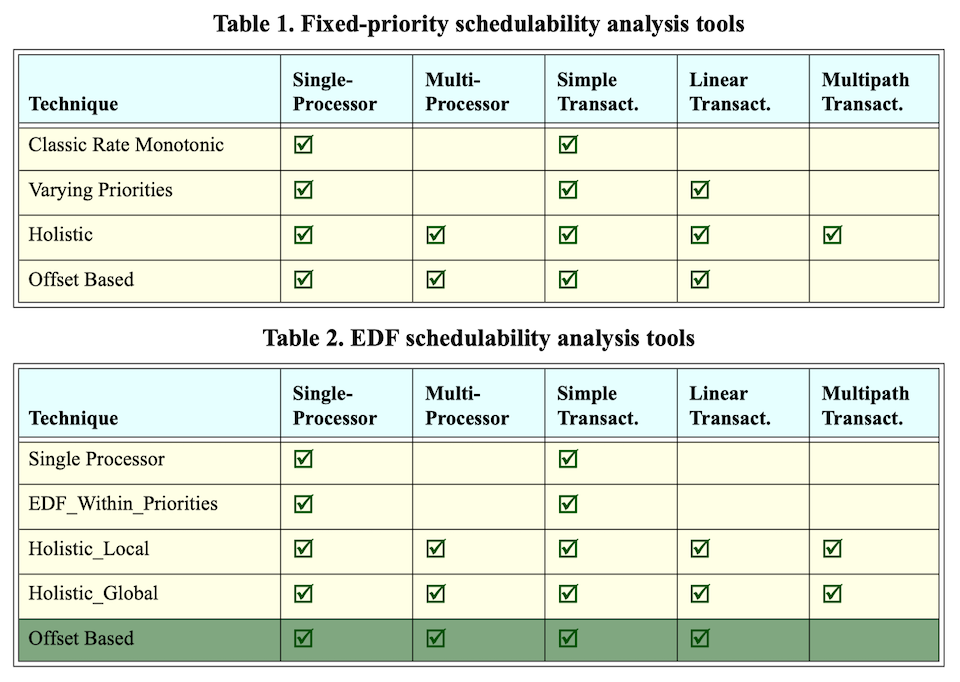
\includegraphics[width=5in]{images/mast-analysis}
\caption{MAST analysis tools \cite{mast-analysis}.}
\label{mast-analysis-tools}
\end{figure}

\begin{itemize}
   \item \textit{Classic RM Analysis}: it implements the classic exact response time analysis for single-processor fixed-priority systems and corresponds to the Technique "Calculating response time with arbitrary deadlines and blocking" in \cite{practitioner}. Although it's called Rate Monotonic, it bases on the final work by Tindell regarding Deadline Monotonic analysis to include jitters \cite{tindell-dm};
   \item \textit{Holistic Analysis}: this analysis extends the response time analysis to multiprocessor and distributed systems. It is not an accurate analysis because it makes the assumption that tasks of the same transaction are independent. It was first developed for fixed priority systems by Tindell and Clark \cite{holistic-analysis}. It has no use for our purposes, but it is worth mentioning to the reader because it can support both FPS and EDF monoprocessor and has fewer restrictions compared to \textit{Classic RM Analysis}, as explained below. In terms of our example application, both techniques provide equivalent results;
   \item \textit{EDF Monoprocessor / Single Processor}: it implements the exact response time analysis for single-processor EDF systems first developed by Spuri \cite{spuri};
   \item \textit{Offset Based Approximate Analysis}: this is a response time analysis for multiprocessor and distributed systems that improves the pessimism of the holistic analysis by taking into account that tasks of the same transaction are not independent, through the use of offsets. Offset based analysis for fixed priorities was first introduced by Tindell \cite{tindell-offsets} and then extended to distributed systems by Palencia and González \cite{pessimistic-rma};
   \item \textit{Offset Based Approximate with Precedence Relations Analysis}: this is an enhancement of the offset based approximate analysis for fixed priority systems in which the priorities of the tasks of a given transaction are used together with the precedence relations among those tasks to provide a tighter estimation of the response times;
   \item \textit{Offset Based Slanted Analysis}: this is another enhancement of the offset based approximate analysis for fixed priority systems in which the maximum interference function is defined with a tighter approximation. This method provides better results that the Offset-Based Approximate Analysis, but it is uncertain if it gets better results than the method with precedence relations.
\end{itemize}

In addition, the analysis tools are subject to different restrictions \cite{mast-restrictions}. The most significant ones are:

\begin{itemize}
   \item \textit{No\_Hard\_Local\_Deadlines}: Hard Local Deadlines cannot be used as Timing Requirements;
   \item \textit{Referenced\_Events\_Are\_External\_Only}: no internal events can be referenced by Global Deadlines;
   \item \textit{Simple\_Transactions\_Only}: checks that every transaction has only a continuous sequence of activities executed by the same server. This restriction is required by the Rate Monotonic analysis and the EDF Monoprocessor analysis;
   \item \textit{Linear\_Plus\_Transactions\_Only}: less restrictive than \textit{Simple\_Transactions\_Only}, checks that every transaction only has one external event and is not multipath, e.g. it has no Multicasts. This restriction is required by the Holistic Analysis and the different Offset based analysis tools;
   \item \textit{Restricted\_Multipath\_Transactions\_Only}: checks that every transaction has a single input event, has no branch elements (Delivery or Query Servers), and has no Rate Divisors. It also checks that the transaction follows the set of allowed constructs mentioned in \cite{mast-restrictions}. This restriction is required by the Holistic analysis.
\end{itemize}

As final note, as of the time of writing, offset-based analysis with EDF tasks fallbacks to holistic analysis \cite{mast-analysis}, which in turn does not support shared resources in EDF yet.

\section{FPS analysis}

We start the analysis with fixed priority scheduling (FPS) and a MAST model which represents the tasks as stand-alone. Later, we will try to more strictly model the formal transactions comprised of dependent tasks.

To check that the system meets the deadlines, it suffices to run it for at least the first hyperperiod amount of time. Assuming sporadic tasks as periodic with a period equal to the minimum interarrival time, which is the worst case, the hyperperiod is $LCM(1, 3, 5) = 15s$. The hyperperiod of a set of tasks is least common multiple of all periods.

\subsection{Independent tasks} \label{independent-tasks}

We start with the Rate Monotonic analysis of the initial system.

\begin{lstlisting}
Optimum Resource Ceilings:
request_buffer =>  7
activation_log =>  11
event_queue =>  241
\end{lstlisting}

A first analysis suggests that smaller values can be used as ceilings for the protected objects Request\_Buffer and Activation\_Log. This possible improvement is expected since the two values are the highest priorities of the tasks Regular\_Producer and External\_Event\_Server, respectively. We leave the ceilings intact nevertheless since the ceiling is required to be an upper bound of the priorities between the tasks that request the resource, not the least upper bound. Having some spare priorities between the task priorities and the ceilings might prove to be useful if we need to separate a task into two distinct tasks with proper offset to better model the application \cite{tindell-offsets}.

\begin{longtable}{llllll}
   \toprule
   Task & WCET \\
   \midrule
   regular\_producer & 0.019333 \\
   on\_call\_producer & 0.007126 \\
   activation\_log\_reader & 0.003582 \\
   \toprule
   \toprule
   Transaction & $R_{max}$ & Slack & Worst blocking time & Jitter \\
   \midrule
   rp\_transaction & 0.020434  & 2470.0\% &  2.000E-06 & 0.001101 \\
   ocp\_transaction & 0.026592 & 10776.6\% & 1.000E-06 & 0.019472 \\
   alr\_transaction & 0.030195 & 26600.8\% & 0.00 & 0.026613 \\
   interrupt\_transaction & 2.102E-05 & >=100000.0\% & 1.000E-06 & 1.102E-05 \\
   \toprule
   \toprule
   System slack & 2401.2\% \\
   Total utilisation & 2.68\% \\
   \bottomrule
\caption{Rate Monotonic analysis results for FPS}
\label{tab:rm-fps}
\end{longtable}

Table \ref{tab:rm-fps} first shows the WCET of the tasks as defined in the MAST model and which are controlled by the Whetstone workloads. Then the results of the analysis are displayed, containing the worst-case response time $R_{max}$, the slack, the blocking time and the jitter for each transaction. The MAST analysis tool also provides best-case response times $R_{min}$, but Rate Monotonic is a pessimistic analysis which assumes worst-case scenario at the critical instant, therefore only worst-case response time matters.

All transactions suffer jitter due to the system ticker interrupt running at the highest interrupt priority and the context switch overhead.

\begin{itemize}
   \item \textit{regular\_producer}: suffers additional jitter due to the system clock with granularity 1ms and the possible execution of the interrupt handler. Its blocking time is caused by the On\_Call\_Producer and the Activation\_Log\_Reader which have lower priorities but can access resources with higher ceiling priority than Regular\_Producer;
   \item \textit{ocp\_transaction}: suffers additional jitter due to interference by Regular\_Producer. Its blocking time is caused by the Activation\_Log\_Reader;
   \item \textit{alr\_transaction}: suffers additional jitter due to interference by On\_Call\_Producer and Regular\_Producer. It has no blocking time since it's the task with the lowest priority;
   \item \textit{interrupt\_transaction}: it's the software level handler of the interrupt. It suffers no additional jitter other than the aforementioned overheads. Its blocking time is caused by the Activation\_Log\_Reader;
\end{itemize}

We shall now increase the Whetstone workload of factor 24 in the first three transactions since 2477.0\% is the smallest slack of the three of them. The factor corresponds to how much the execution time of all event responses can be increased while preserving system schedulability \cite{practitioner-growth}. We leave the {interrupt\_transaction} intact because it doesn't contain any Whetstone operation. The new results are as shown in table \ref{tab:rm-fps-24}.

\begin{longtable}{llllll}
   \toprule
   Task & WCET \\
   \midrule
   regular\_producer & 0.482597 \\
   on\_call\_producer & 0.177482 \\
   activation\_log\_reader & 0.088702 \\
   \toprule
   \toprule
   Transaction & $R_{max}$ & Slack & Worst blocking time & Jitter \\
   \midrule
   rp\_transaction & 0.485486  & 2.73\% &  2.000E-06 & 0.002889 \\
   ocp\_transaction & 0.662657 & 76.95\% & 1.000E-06 & 0.485175 \\
   alr\_transaction & 0.751706 & 277.34\% & 0.00 & 0.663004 \\
   interrupt\_transaction & 2.102E-05 & >=100000.0\% & 1.000E-06 & 1.102E-05 \\
   \toprule
   \toprule
   System slack & 3.21\% \\
   Total utilisation & 57.52\% \\
   \bottomrule
   \caption{Rate Monotonic analysis results for FPS increased of factor 24}
\label{tab:rm-fps-24}
\end{longtable}

The blocking times have not changed because protected operations are the same as before, but the total utilisation has increased up to 57.52\%. The 2.73\% slack value of Regular\_Producer is already very low, so we can leave it as it is. We proceed instead to increase the workload of On\_Call\_Producer and Activation\_Log\_Reader from factor 24 to $43\ =\ 24\ *\ 1.77$, using the slack value 77\%.

\begin{longtable}{llllll}
   \toprule
   Task & WCET \\
   \midrule
   regular\_producer & 0.482597 \\
   on\_call\_producer & 0.312341 \\
   activation\_log\_reader & 0.156086 \\
   \toprule
   \toprule
   Transaction & $R_{max}$ & Slack & Worst blocking time & Jitter \\
   \midrule
   rp\_transaction & 0.485486  & 0.390625\% &  2.000E-06 & 0.002889 \\
   ocp\_transaction & 0.798039 & 0.390625\% & 1.000E-06 & 0.485698 \\
   alr\_transaction & 0.954730 & 28.13\% & 0.00 & 0.798644 \\
   interrupt\_transaction & 2.102E-05 & 15421.1\% & 1.000E-06 & 1.102E-05 \\
   \toprule
   \toprule
   System slack & 0.390187\% \\
   Total utilisation & 64.26\% \\
   \bottomrule
   \caption{Rate Monotonic analysis results for FPS increased of factor 43}
\label{tab:rm-fps-24-ocp-44}
\end{longtable}
 
The system has reached utilisation 64.26\%. We now increase the workload of Activation\_Log\_Reader from factor 43 to $55\ =\ 43 * 1.28$, using the slack value 28\%.

\begin{longtable}{llllll}
   \toprule
   Task & WCET \\
   \midrule
   regular\_producer & 0.482597 \\
   on\_call\_producer & 0.312341 \\
   activation\_log\_reader & 0.198645 \\
   \toprule
   \toprule
   Transaction & $R_{max}$ & Slack & Worst blocking time & Jitter \\
   \midrule
   rp\_transaction & 0.485492  & 0.0\% &  2.000E-06 & 0.002889 \\
   ocp\_transaction & 0.798039 & 0.390625\% & 1.000E-06 & 0.485698 \\
   alr\_transaction & 0.997454 & 0.390625\% & 0.00 & 0.798809 \\
   interrupt\_transaction & 2.102E-05 & 15421.1\% & 1.000E-06 & 1.102E-05 \\
   \toprule
   \toprule
   System slack & 0.390187\% \\
   Total utilisation & 65.68\% \\
   \bottomrule
   \caption{Rate Monotonic analysis results for FPS increased of factor 55}
\label{tab:rm-fps-24-ocp-44-alr-56}
\end{longtable}

The maximum utilisation reached is about 65.68\%. The only transaction with significant slack left is \texttt{interrupt\_transaction}, but tests show that an increase of the WCET of factor 154 in the operation \textit{external\_event\_server} would improve the utilisation only up to 65.71\%, hence we can ignore it.

\subsection{Adding offsets}

So far, tasks have been assumed to be scheduled independently, there are no relationships between the release of any pair of tasks. Consequently, the worst-case task release pattern has been assumed in the critical instants \cite{critical-instants}; the resulting analysis is, therefore, sufficient for any task release pattern. It may, however, be advantageous to specify timing constraints on release patterns. We try to include time offsets into the computational model and, by taking account of time offsets, we try to reduce the pessimism when bounding the timing behaviour of the system.

By assuming all tasks are independent, the current analysis is subject to two pessimistic points:

\begin{enumerate}
   \item Critical instant: for tasks with offsets, we must take into account that the critical instant may not include the simultaneous activation of all higher priority tasks, as it was the case when all tasks were independent. The existence of offsets makes it impossible for some sets of tasks to become active simultaneously \cite{pessimistic-rma};
   \item Blocking time: offsets can be used to avoid the need for a dynamic concurrency control protocol for access to shared resources. Two tasks in the same transaction may not need to use locks to guard access to a shared resource if certain constraints on response times and offsets hold \cite{tindell-offsets}.
\end{enumerate}

The above pessimism can be avoided by modeling the precedence constraint: within a pair of tasks, one of them must complete execution before the other can be permitted to commence. If it can be shown that two tasks execute in exclusion, then any resources shared exclusively between these tasks need not be guarded by locks, the tasks are guaranteed never to access the shared resource concurrently. Besides, the two tasks cannot be active concurrently, which means that neither task can be permitted to preempt the other, causing interference in the critical instant.

\subsubsection{Critical instant}

Offsets can be used to express precedence constraints: the existence of offsets makes it impossible for some sets of tasks to become active simultaneously. This is achieved by "spreading out" the computation of tasks so that all the tasks are not released together.

In our system, the task On\_Call\_Producer (OCP) is actually not truly sporadic given that it's activated by the Regular\_Producer (RP) every 3 jobs. The two tasks are not thus independent and both the RP job which activates OCP and the latter should belong to the same transaction. The equivalent argument holds true for the RP job that awakens Activation\_Log\_Reader (ALR). The remaining instances of the RP tasks should belong to another transaction again.

Formally, with a precedence constraint, for two tasks $\tau_C$ and $\tau_D$ that are members of the same transaction, $\tau_C$ must complete before task $\tau_D$ is run. We have in theory two possible priority situations: task $\tau_C$ is of higher priority, or task $\tau_D$ is of higher priority. Fortunately, in our system, $\tau_C = RP, \tau_D = OCP$ and RP is the one of higher priority, which means that task OCP (of lower priority) will simply not execute if task RP has been released before task OCP and has remaining computation. It can be seen that the condition for the precedence constraint to be met is \cite{tindell-offsets}:

$\Phi_{C}\ +\ J_{C}\ \le\ \Phi_{D} \Leftrightarrow \Phi_{RP}\ +\ J_{RP}\ \le\ \Phi_{OCP}$

Otherwise, if task $\tau_D$ were of higher priority, we could not use the priority mechanism to ensure precedence and would rely on offsets. Therefore, for the precedence relation to hold, the latest finish time of $\tau_C$ must be before the earliest release time of $\tau_D$, i.e.:

$O_C + r_c < O_D$, where $r_c$ is the response time of C

MAST Offset-based analysis tools are able to derive such conditions from the following representations of the newly described transactions.

\begin{figure}[!htbp]
\centering
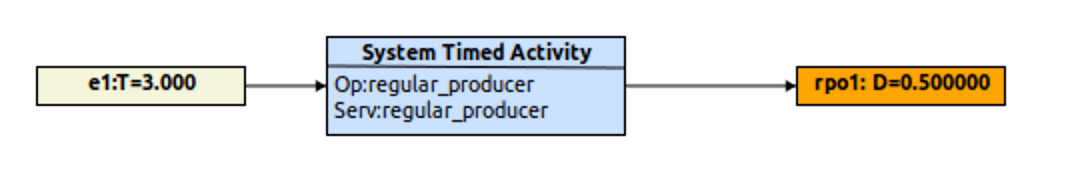
\includegraphics[width=5in]{images/transaction-rp-offset}
\caption{Transaction A}
\label{transaction-rp-offset}
\end{figure}

The transaction A has a period of 3, representing the stand-alone RP instance.

\begin{figure}[!htbp]
\centering
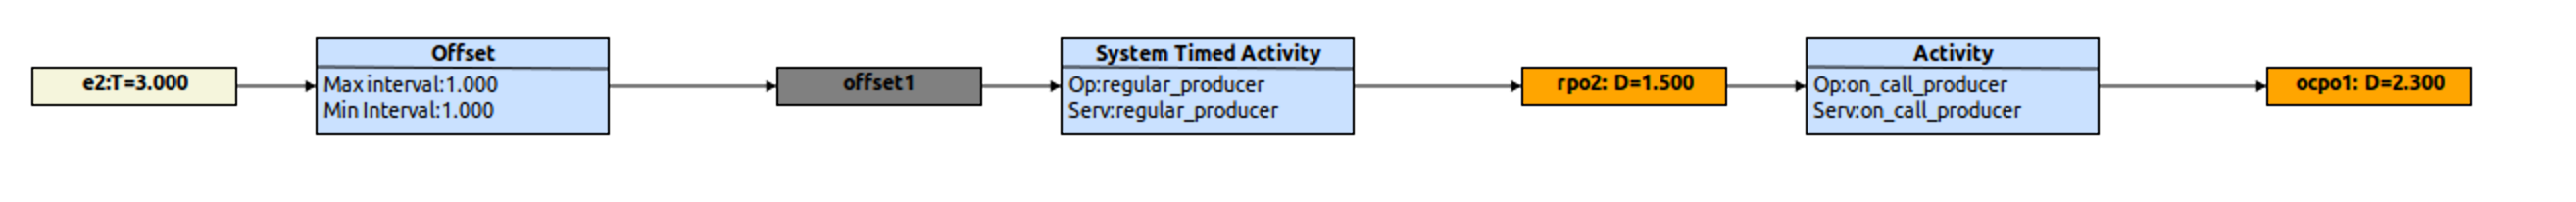
\includegraphics[width=6.5in]{images/transaction-ocp-offset}
\caption{Transaction B}
\label{transaction-ocp-offset}
\end{figure}

\begin{figure}[!htbp]
\centering
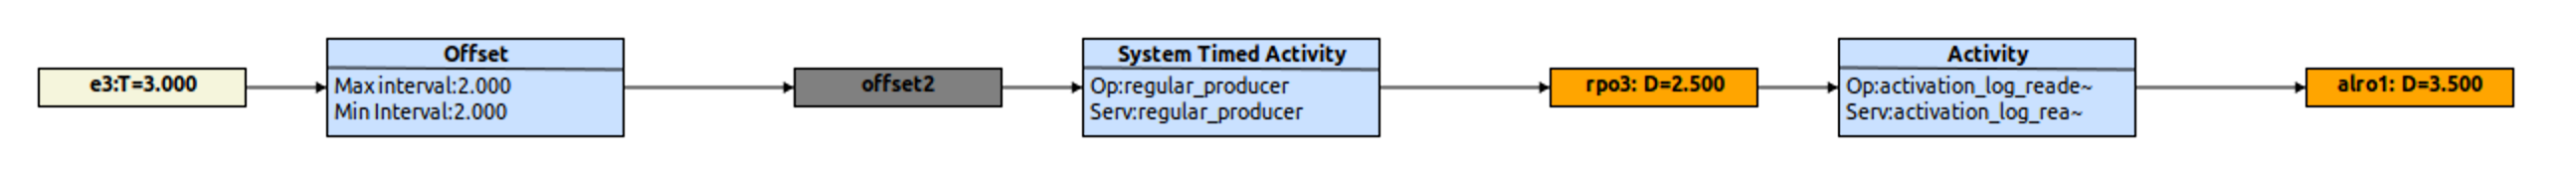
\includegraphics[width=6.5in]{images/transaction-alr-offset}
\caption{Transaction C}
\label{transaction-alr-offset}
\end{figure}

The transactions B and C also have a period of 3 and include the RP job which activates the OCP and ALR jobs respectively. Both transactions have an initial offset from the external periodic event to differentiate each RP instance from the others.

The unfolding of the three transactions reproduces the timeline in Figure \ref{timeline-offsets}, assuming the Whetstone values reached by the previous analysis. It is clear from the timeline that there is a possibility for the OCP and ALR jobs to further expand their executions without provoking any deadline miss. Nevertheless, the pessimistic Rate Monotonic analysis returns zero slack because of the possible interference between stand-alone tasks.

\begin{figure}[!htbp]
\centering
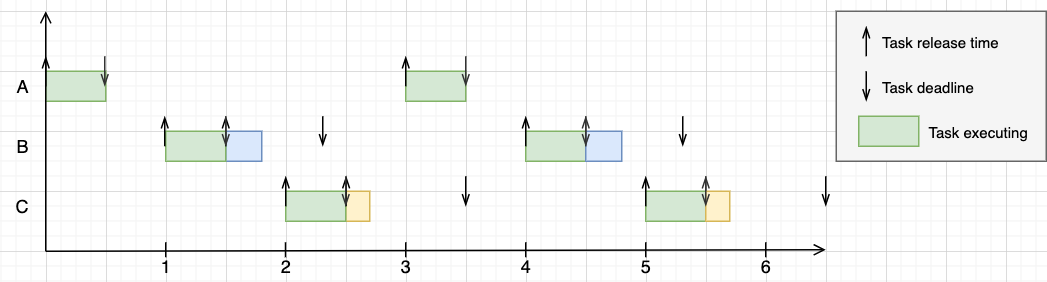
\includegraphics[width=6.5in]{images/timeline-offsets}
\caption{Unfolded timeline}
\label{timeline-offsets}
\end{figure}

As can be seen below, the Offset Based Slanted analysis provides an improvement of the best response times. Offset-based analysis tools are able to consider the offset values, so that chained tasks are not released together.

\begin{longtable}{lllllll}
   \toprule
   Task & WCET \\
   \midrule
   regular\_producer & 0.482597 \\
   on\_call\_producer & 0.312341 \\
   activation\_log\_reader & 0.198645 \\
   \toprule
   \toprule
   Transaction & $R_{min}$ & $R_{max}$ & Slack & Worst blocking time & Jitter \\
   \midrule
   transaction\_a & 0.482597 & 1.454 & -66.02\% &  2.000E-06 & 0.971820 \\
   transaction\_b RP & 1.483 & 2.454 & -66.02\% & 2.000E-06 & 0.971820 \\
   transaction\_b OCP & 1.795 & 3.737 & -66.02\% & 1.000E-06 & 1.942 \\
   transaction\_c RP & 2.483 & 3.454 & -66.02\% & 2.000E-06 & 0.971820 \\
   transaction\_c ALR & 2.681 & 4.936 & -66.02\% & 0.00 & 2.255 \\
   interrupt\_transaction & 1.000E-05 & 2.102E-05 & -100.0\% & 1.000E-06 & 1.102E-05 \\
   \toprule
   \toprule
   System slack & -65.55\% \\
   Total utilisation & 65.68\% \\
   \bottomrule
   \caption{Offset Based Slanted analysis results}
\label{tab:rm-fps-24-ocp-44-alr-56}
\end{longtable}

Both the $R_{min}$ and $R_{max}$ response times produced by the analysis include the initial offsets of the transaction, but the former RP $R_{min}$ values are also used as offset $\Phi_{ij}$ of the dependant tasks OCP and ALR for their own response times. The $R_{max}$ values are instead the sum of the corresponding $R_{min}$ and jitter.

Between $R_{min}$ and $R_{max}$ response times, we consider only the best-case response time $R_{min}$. The timeline in Figure \ref{timeline-offsets} clearly shows that the three transactions have the same source of activation, a RP job, and there is no interference between tasks. Thus there cannot be any significant jitter and only the $R_{min}$ value is valuable for our considerations since it already takes into account the offsets and examines the actual case with zero interference. Besides, by not considering the worst-case response times, we ignore the slack values as well. If the best-case response time is within the deadline, then it's sufficient for our considerations.

\begin{table}[!htbp]
  \centering
  \begin{tabular}{llllll}
   \toprule
   Task & WCET \\
   \midrule
   regular\_producer & 0.482597 \\
   on\_call\_producer & 0.312341 \\
   activation\_log\_reader & 0.198645 \\
   \toprule
   \toprule
   Transaction & $R_{min}$ & $R_{max}$ & Slack & Worst blocking time & Jitter \\
   \midrule
   transaction\_a & 0.482597 & 1.454 & -66.02\% &  2.000E-06 & 0.971820 \\
   transaction\_b RP & 1.483 & 2.454 & -66.02\% & 2.000E-06 & 0.971820 \\
   transaction\_b OCP & 1.795 & \textbf{2.768} & -66.02\% & 1.000E-06 & \textbf{0.973028} \\
   transaction\_c RP & 2.483 & 3.454 & -66.02\% & 2.000E-06 & 0.971820 \\
   transaction\_c ALR & 2.681 & \textbf{3.967} & -66.02\% & 0.00 & \textbf{1.286} \\
   interrupt\_transaction & 1.000E-05 & 2.102E-05 & -100.0\% & 1.000E-06 & 1.102E-05 \\
   \toprule
   \toprule
   System slack & -65.55\% \\
   Total utilisation & 65.68\% \\
  \end{tabular}
  \caption{Offset Based Approximate with Precedence Relations analysis results }
  \label{tab:off-approx-w-pr-fps}
\end{table}

Compared to Offset Based Slanted, Offset Based Approximate with Precedence Relations analysis is able to provide even tighter worst-case response times by using the precedence relation and therefore considering a dynamic offset $\Phi_{i2} \in [R_{ISR\ min}, R_{ISR\ max}]$. I.e. the OCP task is never activated before the RP completion, therefore its jitter can be approximately reduced to $J_{B, OCP} = J_{B, RP}$.

Future analysis in this section will provide only the results from the Offset Based Approximate with Precedence Relations technique, referred only as Offset-based analysis, as it has proved to be the best of the two tools even if are interested only in best-case response times.

\subsubsection{Blocking time}

We can further improve the analysis by reducing unnecessary blocking time: the precedence constraint between the RP and OCP means the former cannot suffer blocking time from the latter. There is also no need to use any lock to guard access to the Request\_Buffer resource given that concurrent access is not possible.

By removing the resource lock on Request\_Buffer, we obtain the results in table \ref{tab:off-approx-w-pr-blocking-time} for the three transactions.

\begin{table}[!htbp]
   \centering
   \begin{tabular}{llll}
    \toprule
    Task & WCET \\
    \midrule
    regular\_producer & 0.482597 \\
    on\_call\_producer & 0.312341 \\
    activation\_log\_reader & 0.198645 \\
    \toprule
    \toprule
    Transaction & $R_{min}$ & Worst blocking time & Jitter \\
    \midrule
    transaction\_a & 0.482597 &  \textbf{1.000E-06} & 0.971820 \\
    transaction\_b RP & 1.483 & \textbf{1.000E-06} & 0.971820 \\
    transaction\_b OCP & 1.795 & 1.000E-06 & \textbf{0.973028} \\
    transaction\_c RP & 2.483 & \textbf{1.000E-06} & 0.971820 \\
    transaction\_c ALR & 2.681 & 0.00 & \textbf{1.286} \\
    interrupt\_transaction & 1.000E-05 & 1.000E-06 & 1.102E-05 \\
    \toprule
    \toprule
    Total utilisation & 65.68\% \\
   \end{tabular}
   \caption{Offset-based analysis without \texttt{request\_buffer}}
   \label{tab:off-approx-w-pr-blocking-time}
 \end{table}

The IPCP ensures that each task can be blocked at most once, at its beginning, by a single lower-priority task \cite{ada-pcp}. Then the removal of the lock on Request\_Buffer reduces the maximum blocking time suffered the tasks to a value equal to the execution time of the lowest priority Activation\_Log\_Reader within the shared resource Activation\_Log.

Further in-depth analysis is presented later in Section \ref{edf-blocking-time}, which gathers the observations for both FPS and EDF blocking times actually suffered by our application.

\subsubsection{Maximum utilisation} \label{maximum-utilisation}

Leveraging the newly defined offset-based model, we can try to achieve maximum system utilisation. By having a look at the unfolded timeline in Figure \ref{timeline-offsets}, it is evident that RP has already reached its maximum workload. However OCP can still increase up to approximately 0.5s and likewise ALR. Bearing in mind the possible jitter caused by the system ticker ($0.5 / 0.001 * 3.844E-06 = 0.001922$), both tasks can raise their execution time way to $0.5 - 0.001922 = 0.498078$.

Actually, compared to the Rate Monotonic Analysis, RP can be increased by a tiny amount to get the WCET up to 0.5s as well. The final offset-based FPS analysis with maximum utilisation is displayed in Table \ref{tab:off-approx-w-pr-max-utilisation}.

\begin{table}[!htbp]
   \centering
   \begin{tabular}{llll}
    \toprule
    Task & WCET \\
    \midrule
    regular\_producer & 0.496961 \\
    on\_call\_producer & 0.497936 \\
    activation\_log\_reader & 0.497844 \\
    \toprule
    \toprule
    Transaction & $R_{min}$ & Worst blocking time \\
    \midrule
    transaction\_a & 0.497003 &  1.000E-06 \\
    transaction\_b RP & 1.497 & 1.000E-06 \\
    transaction\_b OCP & 1.995 & 1.000E-06 \\
    transaction\_c RP & 2.497 & 1.000E-06 \\
    transaction\_c ALR & 2.995 & 0.00 \\
    interrupt\_transaction & 1.000E-05 & 1.000E-06 \\
    \toprule
    \toprule
    Total utilisation & 83.28\% \\
   \end{tabular}
   \caption{Offset-based analysis with max utilisation}
   \label{tab:off-approx-w-pr-max-utilisation}
 \end{table}

All the best-case response times are within the deadlines and the concluding maximum utilisation, with proven runtime feasibility, of the FPS system is approximately 83.28\%. If we flatten the final transactions onto a single timeline, we obtain Figure \ref{timeline-flatten}. Within the hyperperiod of 3 seconds, or equivalently 6 blocks of 0.5seconds, there is only a single block of 0.5s of task idleness. The theoretical utilisation is then $5 / 6 = 0.8\bar{3}\%$, very close to the value provided by the MAST analysis.

\begin{figure}[!htbp]
   \centering
   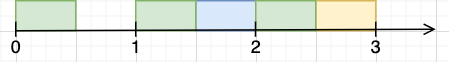
\includegraphics[width=3in]{images/timeline-flatten}
   \caption{Flattened timeline}
   \label{timeline-flatten}
   \end{figure}

Analytically the system utilisation is approximately $\sum_{i \in \{RP, OCP, ALR\}}{C_i \over T_i} = {0.5 \over 1} + {0.5 \over 3} + {0.5 \over 3} = {5 \over 6}$. Runtime overhead, such as system ticker or context switch, and also blocking times have been left out the formula given that they are negligible in the approximation.

\section{EDF Analysis}

The Earliest Deadline First (EDF) \cite{fps-vs-edf} scheduling is dynamic-priority algorithm that assigns priorities to individual jobs of a task based on its absolute deadline.
In particular, the earlier the deadline, the higher the priority.
The absolute deadline of a job is computed as the sum of its release event plus its relative deadline. Such relative deadline is a static attribute, missing in FPS algorithm and corresponding to the maximum response time allowed to each task instance.

The runtime we have adopted is an Ada Ravenscar runtime variant implementing an EDF scheduling coupled with the Deadline Floor Protocol (DFP) \cite{resource-sharing} as resource locking policy.

DFP is the EDF counterpart of the Immediate Priority Ceiling Protocol (IPCP), outlined in Section \ref{the-application}. Indeed, rather than assigning a ceiling priority to each shared resource $r_i$, a deadline floor value $D^i$ is computed as the minimum relative deadline of any task accessing such resource.

Besides, instead of raising the priority of a task to the resource's ceiling, when a task $\tau_i$ released at time $s$ accesses resource $r_i$ at time $t$ (so $s < t$) its relative deadline is immediately reduced to $D^i$. As a result, its active absolute deadline $d_i$ is also (potentially) reduced to $d_i \leftarrow min\{t + D^i, s + D_i\}$. Finally, when the task frees the resource, its deadline immediately returns to its original value.

Clearly, the IPCP for fixed-priority systems and DFP for dynamic-priority systems are structurally equivalent. FPS uses a ceiling value as dispatching urgency, whereas a floor value is expected as earlier deadline under EDF.

\subsection{A MAST model for EDF}

Unfortunately, as mentioned in Section \ref{mast-analysis}, MAST requires even stricter restrictions for EDF analysis tools than FPS. The Offset-based analysis is not yet available for EDF at the time of writing and rollbacks to the Holistic analysis, which in turn does not yet support shared resources. Therefore, we had to discard both Offset-based and Holistic analysis tools.

The last standing option was the EDF Monoprocessor tool, which implements the exact response time analysis for single-processor in EDF systems. Unfortunately, the \textit{Simple\_Transaction\_Only} restriction (§\ref{mast-analysis}) forbids definining a transaction comprising a sequence of activities executed by different Execution Servers. Hence, dependency constraints between the task releases could not be expressed.

In addition, the EDF Monoprocessor analysis is able to support only Stack Resource Policy (SRP) \cite{resource-sharing} as resource access protocol. Under SRP, each job is assigned a preemption level $\pi(\tau_i)$ inversely proportional to the task relative deadline $D_i$, e.g. $\pi(\tau_i) < \pi(\tau_j) \Leftrightarrow D_i > D_j$.

In turn, each resource is assigned a ceiling preemption level $\Pi(r_i)$ defined as the maximum preemption level of any job that may access it. After defining the system ceiling $\hat{\pi}$ as the highest ceiling of all the resources which are held by some job at any time $t$, the following definition of the SRP locking policy is provided. A job $j_i$ released at time $t$ can start execution only if:

\begin{itemize}
   \item the absolute deadline of this job ($t + D_i$) is the earliest deadline of the active requests in the task set;
   \item its preemption level is higher than the system ceiling $\pi(r_i) > \hat{\pi}$.
\end{itemize}

Nevertheless, the disparity in resource access control protocols between runtime implementation and MAST can be ignored because of
the worst-case bound equivalence between SRP and DFP \cite{resource-sharing}. Indeed they lead to even the same worst blocking time analysis.

As a result, within the MAST model, we must provide the preemption level for each task according to the SRP. An available assignment is displayed in Table \ref{tab:preemption-levels}.

\begin{table}[!htbp]
   \centering
   \begin{tabular}{lcc}
     \toprule
     Task name & Deadline (ms) & Preemption Level \\
     \midrule
     External\_Event\_Server & 100 & 40 \\
     Regular\_Producer & 500 & 30 \\
     On\_Call\_Producer & 800 & 20 \\
     Activation\_Log\_Reader & 1000 & 10 \\
     \bottomrule
   \end{tabular}
   \caption{Preemption Levels for the task set}
   \label{tab:preemption-levels}
\end{table}

According to the newly defined preemption levels, Table \ref{tab:ceiling-preemption-level} shows a correct definition of the resource ceilings.

\begin{table}[!htbp]
   \centering
   \begin{tabular}{lc}
     \toprule
     Resource name & Ceiling Preemption Level \\
     \midrule
     Request\_Buffer & 30 \\
     Activation\_Log & 40 \\
     Event\_Queue & 50 \\
     \bottomrule
   \end{tabular}
   \caption{Ceiling Preemption Levels for the resource set}
   \label{tab:ceiling-preemption-level}
\end{table}

\subsection{EDF Monoprocessor analysis}

The EDF Monoprocessor tool is based on the formal analysis developed by Spuri \cite{spuri}, which considers the busy period to study the feasibility of the schedule. As depicted in Figure \ref{fig:spuri}, the worst-case response time (WCRT) of a task $\tau_i$ is found in a busy period $[t_{1},t_{2}]$ in which all other tasks are released synchronously at $t=0$ and then at their maximum rate. Such busy period is characterized by the job $j_i$ released at time $t=a$, $a \ge 0$, preceded by other jobs of any task which do not let the CPU idle, possible by other instances of task $\tau_i$ itself. $t_1$ is the first instant preceding the release of $j_i$ without CPU idleness, whereas $t_{2}$ is the completion time of the job $i$ under consideration.

\begin{figure}[!htbp]
   \centering
   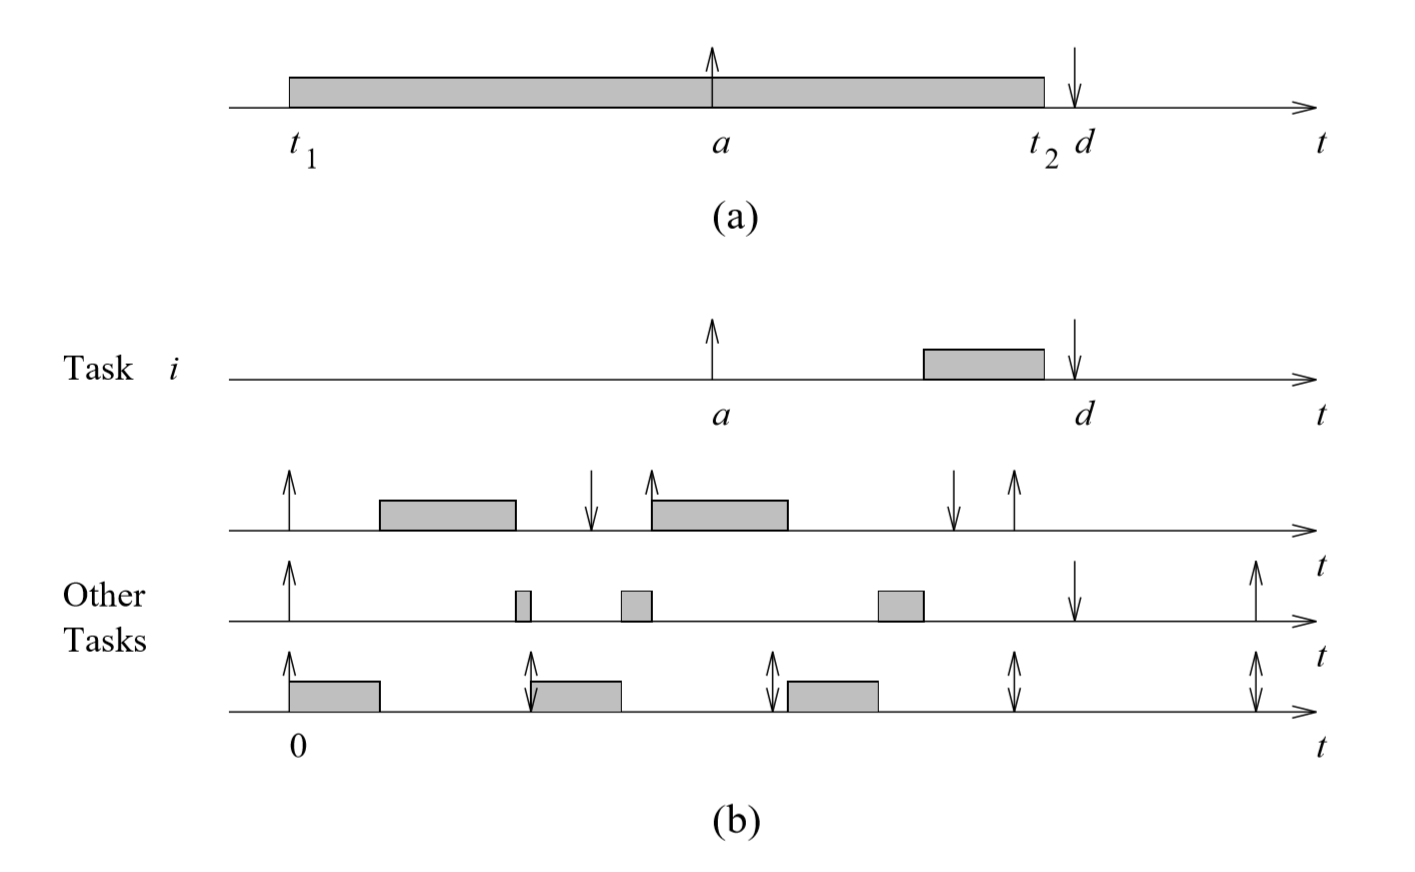
\includegraphics[width=5in]{images/spuri}
   \caption{Busy period (a) leading to the job $j_i$ WCRT (b) \cite{spuri}}
   \label{fig:spuri}
\end{figure}

With this being said, the transactions of this model are precisely those in the FPS model with the independent task set as outlined in §\ref{independent-tasks}. Thus we still have four transactions, each one composed of a single activity.

As workload values, we have set the best values reached by the Offset-based analysis and fed the model to the EDF Monoprocessor analysis to compare the two tools. The results for the latter are pasted in Table \ref{tab:EDF-monoprocessor}.

\begin{table}[!htbp]
   \centering
   \begin{tabular}{lllcl}
    \toprule
    Task & WCET \\
    \midrule
    regular\_producer & 0.496961 \\
    on\_call\_producer & 0.497936 \\
    activation\_log\_reader & 0.497844 \\
    \toprule
    \toprule
    Transaction & $R_{max}$ & Slack & Worst blocking time & Jitter \\
    \midrule
    rp\_transaction        & 0.992883  & -99.22\%   & 2.000E-06  & 0.495880 \\
    ocp\_transaction       & 1.293     & -99.22\%   & 2.000E-06  & 0.794917 \\
    alr\_transaction       & 1.493     & -100.00\%  & 2.000E-06  & 0.995006 \\
    interrupt\_transaction & 0.592882  & -100.00\%  & 1.000E-06  & 0.592872 \\
    \toprule
    \toprule
    System slack & -32.98\% \\
    Total utilisation & 82.90\% \\
   \end{tabular}
   \caption{EDF monoprocessor analysis results}
   \label{tab:EDF-monoprocessor}
 \end{table}

As expected, this is an unfair comparison because a busy period in which all tasks but one are released synchronously leads to a great pessimism in the worst-case response time. Figure \ref{fig:timeline-WCRT-RP} presents the worst arrival pattern considered by MAST to cause the WCRT of Regular\_Producer. However, because of the dependencies between release events, RP will never compete for the CPU with ALR because it is the completion of the former which provokes the release event of latter and without overloading the two tasks are never active simultaneous.

\begin{figure}[!htbp]
   \centering
   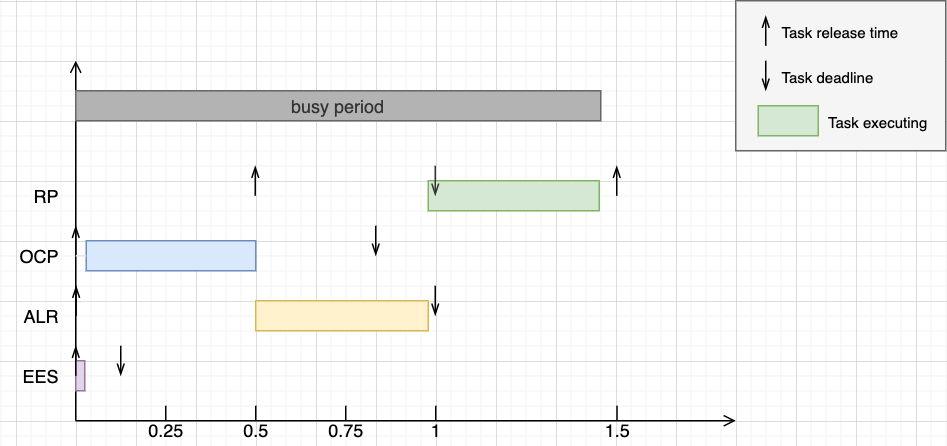
\includegraphics[width=6in]{images/timelines-WCRT-RP}
   \caption{Busy period leading to RP's WCRT}
   \label{fig:timeline-WCRT-RP}
\end{figure}

A more fair comparison would pick Rate Monotonic analysis as the FPS counterpart as response time analysis tool for single-processor since both assume tasks to be standalone. Indeed, providing the best workloads achieved previously via Rate Monotonic, EDF Monoprocessor prints the results in Table \ref{tab:EDF-mono-rate-mono}. The slack values are close to the previous FPS results and the reason can be found again in Figure \ref{fig:timeline-WCRT-RP}. Assuming this pessimistic case, no further significant improvement can be made to any task workload without missing a deadline.

We believe instead that the slight slack improvement is due to the absence of the system ticker in EDF analysis, that is it doesn't take into account the possible release jitters and interferences suffered by each task.

\begin{table}[!htbp]
   \centering
   \begin{tabular}{lllcl}
    \toprule
    Task & WCET \\
    \midrule
    regular\_producer & 0.482555     \\
    on\_call\_producer & 0.312311     \\
    activation\_log\_reader & 0.198612 \\
    \toprule
    \toprule
    Transaction & $R_{max}$ & Slack & Worst blocking time & Jitter \\
    \midrule
    rp\_transaction        & 0.494969  & 0.781250\% & 2.000E-06  & 0.012372 \\
    ocp\_transaction       & 0.794969  & 1.56\%     & 2.000E-06  & 0.482628  \\
    alr\_transaction       & 0.993620  & 3.13\%     & 2.000E-06  & 0.794975   \\
    interrupt\_transaction & 0.094968  & 41928.5\%  & 1.000E-06  & 0.094958    \\
    \toprule
    \toprule
    System slack & 0.783430\% \\
    Total utilisation & 65.29\% \\
   \end{tabular}
   \caption{EDF Monoprocessor analysis results}
   \label{tab:EDF-mono-rate-mono}
 \end{table}

To sum up, MAST can ensure a relatively poor utilisation under EDF scheduling because we aren't allowed to maintain consistency between model and application.
We may question what the real performance granted by such dynamic-scheduling is..

\subsection{Runtime behaviour}

Despite the pessimistic MAST analysis results, EDF is an optimal scheduler and can handle a total theoretic utilisation up to 1. In addition, any feasible preemptive FPS schedule can be transformed into an EDF schedule without affecting its feasibility \cite{spuri}. Hence, we expect the EDF runtime to perform at least as well as the FPS counterpart under the maximum workload reached with Offset-based analysis §\ref{maximum-utilisation}.

\begin{figure}[!htbp]
   \centering
   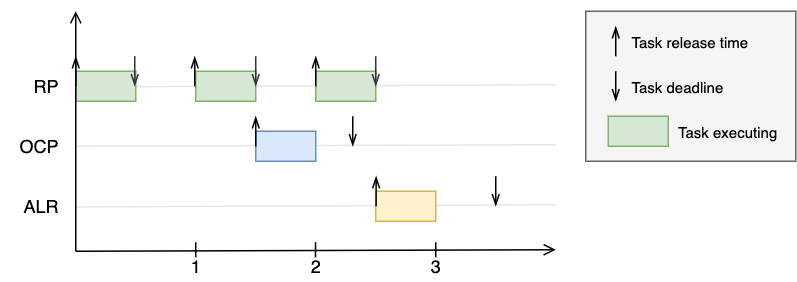
\includegraphics[width=6in]{images/timeline-edf-offsets}
   \caption{Application execution under EDF scheduling with maximum utilisation}
   \label{fig:timeline-edf-offsets}
\end{figure}

Figure \ref{fig:timeline-edf-offsets} exhibits the schedule produced by EDF up to the hyperperiod $H=3$. The total utilisation of 83.28\% is given by the Whetstone values in Table \ref{tab:Whet-max-util}.

\begin{table}[!htbp]
   \centering
   \begin{tabular}{lllcl}
    \toprule
    Task & WCET \\
    \midrule
    regular\_producer & 0.496961     \\
    on\_call\_producer & 0.497936     \\
    activation\_log\_reader & 0.497844 \\
    \toprule
   \end{tabular}
   \caption{Whetstone values leading to maximum FPS and EDF utilisation}
   \label{tab:Whet-max-util}
 \end{table}

\newpage

Despite the EDF optimality, by observing the aforementioned timeline, there is, unfortunately, no room for utilisation increase. RP already runs at zero laxity, whereas OCP and ALR cannot exceed an execution time of 0.5 seconds without causing a fatal release jitter to RP itself.

This is further proved by noting that both EDF and FPS algorithms lead to the same schedule of our application, under the condition that no task misses its deadline. FPS assigns priorities inversely proportional to the relative deadline $D_i$, whereas EDF calculates them inversely proportional to the absolute deadline $d_i$. In general, the relation $D_i < D_j \Leftrightarrow d_i < d_j$ does not hold, but in our specific case we can demonstrate it's valid.

Given a pair of task $\tau_i$ and $\tau_j$, for the task $\tau_i$ with relative deadline $D_i > D_j$ to have absolute deadline $d_i < d_j$ it must be released at time $t_i < t_j$, i.e. for OCP to have a lower absolute deadline than RP. But under the condition that no task overruns, this situation is clearly not possible. Both OCP and ALR are always activated by the RP, and they complete before the next release of RP. This proves that, within our application with precedence relations, $D_i < D_j \Leftrightarrow d_i < d_j$ and therefore both algorithms assign the same priority.

We provide further proof of the equivalence between FPS and EDF scheduling by observing the execution metrics. We have enhanced both runtimes with custom instrumentation to provide valuable execution information such as deadline misses, execution counts, preemptions and release jitters.

\begin{table}[!htbp]
   \centering
   \begin{tabular}{lllllll}
    \toprule
    Task & DM & Exec & Preempt & Min Release Jitter & Max Release Jitter & $R_{max}$ \\
    \midrule
    Regular\_Producer & 0 & 19 &  0 & 0.001053733 &  0.001505544 & 0.498750639 \\
    On\_Call\_Producer & 0 & 6 &  0 & 0.000033067 &  0.000034194 & 0.498277889 \\
    Activation\_Log\_Reader & 0 & 6 &  0 & 0.000032178 &  0.000033528 & 0.494317389 \\
    \toprule
    Total utilisation & 83.33\% \\
    \toprule
   \end{tabular}
   \caption{Instrumentation values for FPS schedule with maximum utilisation}
   \label{tab:instrumentation-fps-050}
 \end{table}

Table \ref{tab:instrumentation-fps-050} provides the results for the FPS execution with the system under maximum utilisation, up to 19 executions of Regular\_Producer. No job misses its deadline nor suffers preemption since executions never overlap. Release jitter is skipped for External\_Event\_Server since it's always the task with highest priority and it's not periodic, thus not subject to System Tick granularity.

\begin{table}[!htbp]
   \centering
   \begin{tabular}{lllllll}
    \toprule
    Task & DM & Exec & Preempt & Min Release Jitter & Max Release Jitter & $R_{max}$ \\
    \midrule
    Regular\_Producer & 0 & 19 & 0 & 0.001056517 & 0.001313233 & 0.497775894 \\
    On\_Call\_Producer & 0 & 6 & 0 & 0.000029317 & 0.000030450 & 0.503115856 \\
    Activation\_Log\_Reader & 0 & 6 & 0 & 0.000031033 & 0.000032261 & 0.499129944 \\
    \toprule
    Total utilisation & 83.33\% \\
    \toprule
   \end{tabular}
   \caption{Instrumentation values for EDF schedule with maximum utilisation}
   \label{tab:instrumentation-edf-050}
 \end{table}

Table \ref{tab:instrumentation-edf-050} displays the analogous results for the EDF schedule. Basically, the two runtimes lead to the same behaviour and any difference in jitter is negligible.

Results with less workload are equivalent in both FPS and EDF cases.

\subsection{Blocking Time}\label{edf-blocking-time}
Further consideration can be made about the blocking time by reasoning with the timeline in Figure \ref{fig:timeline-edf-offsets}. The blocking time suffered by each job is equal to zero, except for one case, for that no higher-priority job will be suspended waiting for a lower-priority job to complete its use of a (non-preemptable) resource.

Since DFP is structurally equivalent to IPCP, there are two kinds of possible blocking \cite{ada-pcp}.

\begin{enumerate}
   \item Direct blocking, a situation in which a higher priority task is blocked by a lower-priority task which accesses a resource shared between the two of them. In our application, this may happen only between ALR and External\_Event\_Server (EES), which have independent release events. Direct blocking cannot happen between RP and OCP, again because they are never simultaneously active;
   \item Push-through blocking happens when a medium priority task can be blocked by a lower priority task, which inherits the priority of a high priority task. In our analysis, the only plausible case would be RP being push-blocked by ALR, which receives the priority of EES. However, since ALR is activated when RP terminates and vice versa, this situation cannot happen between the two tasks.
\end{enumerate}

Because of the comparability between PCP and DFP and the schedule correspondence between FPS and EDF with our taskset, the aforementioned observations about the blocking time can also be made for the fixed-priority application.

\section{Overloading}

A job is said to overrun when it executes for more than its guaranteed execution time. We say that a system is overloaded when it is not schedulable on the basis of the maximum execution times of its tasks, and hence it is likely that some jobs will miss their deadlines \cite{liu-overload}.

Any algorithm for scheduling jobs with potential for overrun should meet two criteria if it is to perform well. First, it should guarantee that jobs which do not overrun meet their deadlines and, second, the algorithm tries to maximise the number of deadlines met.

In this section, we compare the behaviour of our application under FPS and EDF during permanent overload situations, which occur in literature when the system utilisation $U > 1$. In our case, our limit is not the theoretical full CPU utilisation 1, we have seen we should consider 0.83 as limits for both FPS and EDF.

\subsection{FPS overloading}

When tasks have fixed priorities, overruns of jobs in a task can never affect higher-priority tasks, and it is possible to predict which tasks will miss their deadlines during an overload. Likewise, another equivalent point of view is that a permanent overload may cause a complete blocking of the lower priority tasks.

We have observed this behaviour in our tests by increasing the RP workload of a small amount $\epsilon = 0.02s$, reaching a WCET of approximately 0.52s.

\begin{lstlisting}
Interrupt generated
Deadline Miss Detected -  RP
End of cyclic activation.
Deadline Miss Detected -  RP
End of cyclic activation.
Deadline Miss Detected - OCP
Deadline Miss Detected -  RP
End of cyclic activation.
End of sporadic activation.
Deadline Miss Detected -  RP
End of cyclic activation.
Deadline Miss Detected - ALR
End of parameterless sporadic activation.         1
\end{lstlisting}

\begin{figure}[!htbp]
\centering
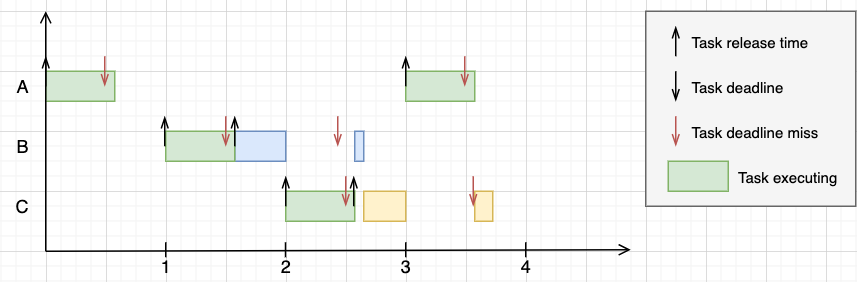
\includegraphics[width=6.5in]{images/timeline-overload-fps-rp}
\caption{Timeline with overruning RP}
\label{timeline-overload-fps-rp}
\end{figure}

As proved by the runtime log and shown in the timeline in Figure \ref{timeline-overload-fps-rp}, an overruning RP affects all the lower-priority tasks and causes their deadline miss as well. The behaviour in the timeline is even more evident by having a look at the runtime instrumentation metrics in Table \ref{tab:instrumentation-fps-052}. All of the OCP and ALR executions miss their respective deadlines and suffer preemptions by RP instances. Besides, ALR also suffers increasing release jitter due to delayed OCP jobs.

\begin{table}[!htbp]
   \centering
   \begin{tabular}{lllllll}
    \toprule
    Task & DM & Exec & Preempt & Min Release Jitter & Max Release Jitter & $R_{max}$ \\
    \midrule
    Regular\_Producer & 19 & 19 & 0 &  0.001053628 &  0.001547378 & 0.524420933 \\
    On\_Call\_Producer & 6 & 6 & 6 &  0.000042828 &  0.000044033 & 1.021757094 \\
    Activation\_Log\_Reader & 6 & 6 & 6 &  0.021249300 &  0.021490806 & 1.039471794 \\
    \toprule
    Total utilisation & 85.33\% \\
    \toprule
   \end{tabular}
   \caption{Instrumentation values for FPS schedule with RP overloading of $\epsilon=0.02$}
   \label{tab:instrumentation-fps-052}
 \end{table}

\begin{lstlisting}
Interrupt generated
End of cyclic activation.
End of cyclic activation.
Deadline Miss Detected - OCP
End of cyclic activation.
Elapsed time: 0.530376517
End of sporadic activation.
End of cyclic activation.
Deadline Miss Detected - ALR
End of parameterless sporadic activation.         1
\end{lstlisting}

\begin{figure}[!htbp]
\centering
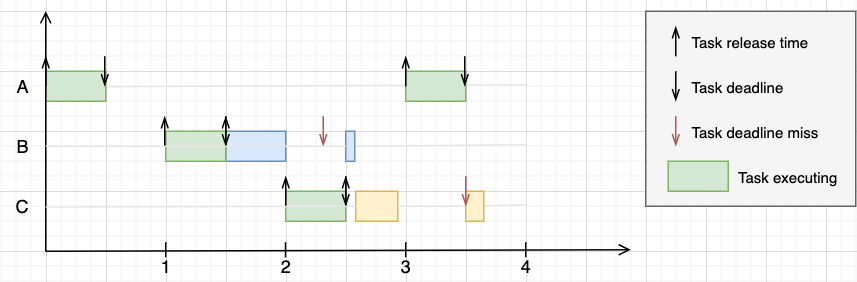
\includegraphics[width=6.5in]{images/timeline-overload-fps-ocp}
\caption{Timeline with overruning OCP}
\label{timeline-overload-fps-ocp}
\end{figure}

Runtime log and Figure \ref{timeline-overload-fps-ocp} show that an overload of OCP never impacts the higher-priority task RP which can meet all its deadlines. ALR will instead miss its deadline once again.

\subsection{EDF overloading}

In literature, the EDF exhibits an unstable behaviour during an overload: a late EDF job which has already missed its deadline has a higher priority than a job whose deadline is still in the future. Consequently, if the execution of a late job is allowed to continue, it may cause the other jobs to be late.

\begin{lstlisting}
Interrupt generated
Deadline Miss Detected -  RP
End of cyclic activation.
Deadline Miss Detected -  RP
End of cyclic activation.
End of sporadic activation.
Deadline Miss Detected -  RP
End of cyclic activation.
Deadline Miss Detected -  RP
End of cyclic activation.
Deadline Miss Detected - ALR
End of parameterless sporadic activation.         1
\end{lstlisting}

\begin{figure}[!htbp]
\centering
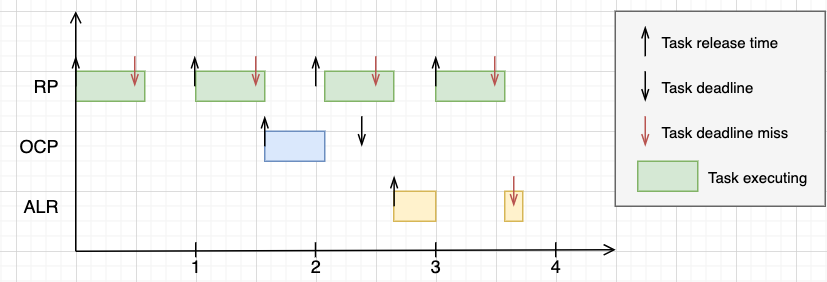
\includegraphics[width=6.5in]{images/timeline-overload-edf-rp}
\caption{Timeline with overruning RP in EDF}
\label{timeline-overload-edf-rp}
\end{figure}

A RP overload of $\epsilon = 0.02s$ causes the deadline miss of the ALR, as shown in the runtime log and Figure \ref{timeline-overload-edf-rp}, but OCP seems to meet its deadline nevertheless. Instrumentation metrics in Table \ref{tab:instrumentation-edf-052} confirm our analysis: OCP has zero deadline misses.

\begin{table}[!htbp]
   \centering
   \begin{tabular}{lllllll}
    \toprule
    Task & DM & Exec & Preempt & Min Release Jitter & Max Release Jitter & $R_{max}$ \\
    \midrule
   Regular\_Producer & 19 & 19 & 0 &  0.001056522 &  0.019908256 & 0.561066067 \\
   On\_Call\_Producer & 0 & 6 & 0 & 0.000038889 &  0.000040044 & 0.503191217 \\
   Activation\_Log\_Reader & 6 & 6 & 6 &  0.000040717 &  0.000041944 & 1.027671206 \\
    \toprule
    Total utilisation & 85.33\% \\
    \toprule
   \end{tabular}
   \caption{Instrumentation values for EDF schedule with RP overloading of $\epsilon=0.02$}
   \label{tab:instrumentation-edf-052}
 \end{table}

This behaviour is apparently in contrast with the FPS overload with the same overruning task. However, if we consider a more significant overrun of $\epsilon = 0.2$ and expand the timeline beyond the hyperperiod, an interesting pattern emerges.

\begin{figure}[!htbp]
\centering
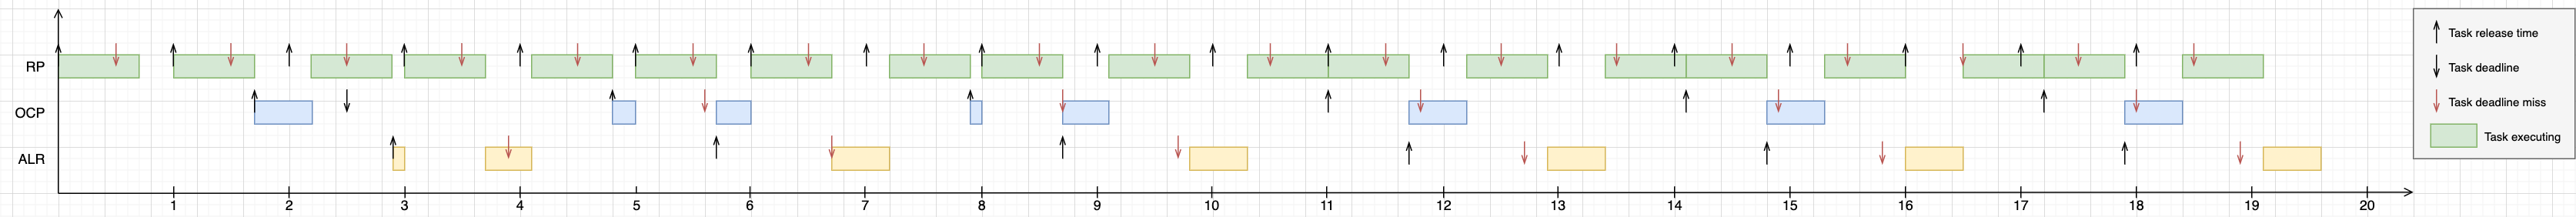
\includegraphics[width=6.5in]{images/timeline-overload-edf-extended}
\caption{Extended timeline with overruning RP in EDF}
\label{timeline-overload-edf-extended}
\end{figure}

All OCP jobs, except for the first instance, fail to meet the deadline and a regular pattern comprising the three tasks emerges as soon as the timeline goes beyond time instant 10. As time elapses from the first activation, OCP and ALR suffer an increasing interference from the overruning RP until time 10, beyond which the jitter is regular. Table \ref{tab:instrumentation-edf-070} provides the evidence: OCP misses all the deadlines but one. Compared to the timeline, the actual execution registers more preemptions for both OCP and ALR. This is due to the fact that the timeline assumes perfect execution times of 0.7s, 0.5s, 0.5s for RP, OCP and ALR respectively. Unfortunately, the real jobs have a slightly less workload which allows OCP and ALR to run for a very brief instant before being preempted by RP.

\begin{table}[!htbp]
   \centering
   \begin{tabular}{lllllll}
    \toprule
    Task & DM & Exec & Preempt & Min Release Jitter & Max Release Jitter & $R_{max}$ \\
    \midrule
    Regular\_Producer & 19 & 19 & 0 &  0.001056522 &  0.237997678 & 1.126713644 \\
    On\_Call\_Producer & 5 & 6 & 5 &  0.000039511 &  0.000040083 & 1.197857533 \\
    Activation\_Log\_Reader & 6 & 6 & 3 &  0.000041700 &  1.105315111 & 1.696978956 \\
    \toprule
    Total utilisation & 100.03\% \\
    \toprule
   \end{tabular}
   \caption{Instrumentation values for EDF schedule with RP overloading of $\epsilon=0.20$}
   \label{tab:instrumentation-edf-070}
 \end{table}

This peculiar EDF behaviour, where there is an initial interval of irregularity followed by regular executions and events, is not exhibited by the analogous FPS algorithm with RP overruning of the same amount. In fixed-priority scheduling, all jobs miss their deadline, and the regularity emerges from the first instant of execution, as in Figure \ref{timeline-overload-fps-extended}. However, Table \ref{tab:instrumentation-fps-070} presents a significant difference between FPS and EDF behaviours from the perspective of ALR. With EDF schedule, ALR is still able to keep the pace and have the same number of executions of OCP. In FPS, ALR suffers much more preemptions from higher-priority tasks and struggle to complete its jobs.

\begin{figure}[!htbp]
\centering
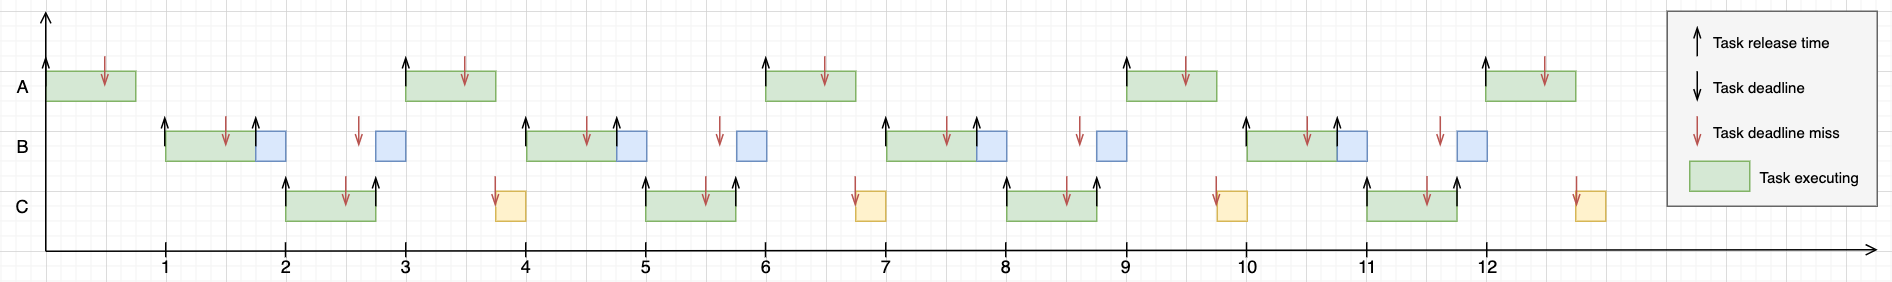
\includegraphics[width=6.5in]{images/timeline-overload-fps-extended}
\caption{Extended timeline with overruning RP in FPS}
\label{timeline-overload-fps-extended}
\end{figure}

\begin{table}[!htbp]
   \centering
   \begin{tabular}{lllllll}
    \toprule
    Task & DM & Exec & Preempt & Min Release Jitter & Max Release Jitter & $R_{max}$ \\
    \midrule
     Regular\_Producer & 19 & 19 & 0 & 0.001053700 & 0.001516400 & 0.698694417 \\
     On\_Call\_Producer & 6 & 6 & 6 & 0.000041728 & 0.000042822 & 1.195951244 \\
     Activation\_Log\_Reader & 4 & 4 & 12 & 0.243860556 & 1.219195511 & 3.281164544 \\
    \toprule
    Total utilisation & 100.03\% \\
    \toprule
   \end{tabular}
   \caption{Instrumentation values for FPS schedule with RP overloading of $\epsilon=0.20$}
   \label{tab:instrumentation-fps-070}
 \end{table}

When the first task that misses its deadline causes all subsequent tasks to miss their deadlines, the effect is called \textit{the domino effect} \cite{value-deadline}. EDF is prone to the domino effect, and it rapidly degrades its performance during overload intervals. This is due to the fact that EDF gives the highest priority to those processes that are close to missing their deadlines. Even worse, we note that a late job which has already missed its deadline has a higher priority than a job whose deadline is still in the future \cite{fps-vs-edf}.

The application under consideration doesn't seem to provoke domino effect. Although a permanent overload of RP causes all subsequent tasks to miss their deadline, it's trivial to show with a timeline that a transient overload of it causes a finite amount of subsequent deadline misses. Eventually, the system is able to recover as long as the system utilisation is below 1. The same property holds for an overruning OCP, as made evident by Figure \ref{timeline-overload-edf-ocp}. We believe this is again because of the precedence relationships. Even if RP misses a deadline, the later OCP and ALR are not activated independently. They wait for RP completion and are less subject to domino effect.

Nevertheless, a difference between FPS and EDF is that, under the former, an overrun in a task cannot cause tasks with higher priority to miss their deadlines but at the expense of lower-priority tasks like ALR. On the contrary, under EDF any other task could miss its deadline, but it is fairer. That is, the latter does not provide any type of guarantee on which tasks will meet their timing constraints, but each task is able to keep the pace.

\begin{figure}[!htbp]
\centering
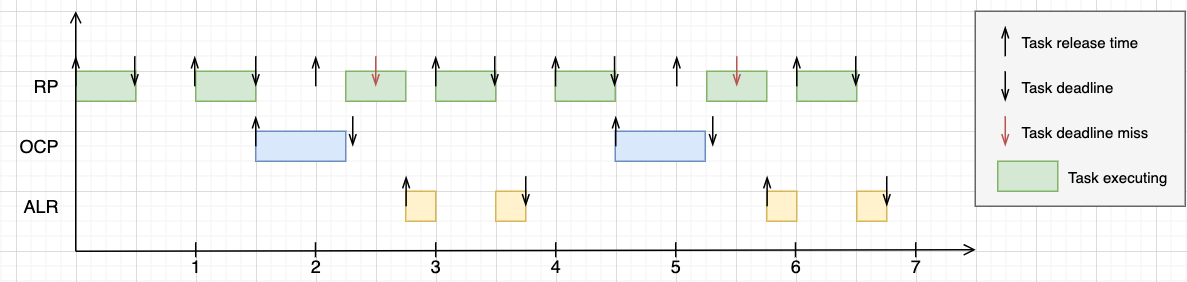
\includegraphics[width=6.5in]{images/timeline-overload-edf-ocp}
\caption{Timeline with overruning OCP in EDF}
\label{timeline-overload-edf-ocp}
\end{figure}

Lastly, an additional interesting property of EDF during permanent overloads is that it automatically performs a period rescaling, and tasks start behaving as they were executing at a lower rate \cite{buttazzo-rm-edf}. The following theorem has been proven by Celvin et al. (2002) \cite{cervin}:

\textit{Assume a set of $n$ periodic tasks, where each task is described by a fixed period $T_i$, a fixed execution time $C_i$, a relative deadline $D_i$, and a release offset $\Phi_i$. If U > 1 and tasks are scheduled by EDF, then the average period $\tilde{T}_i$ of each task $\tau_i$ is given by $\tilde{T}_i = T_iU$.}

With our previous overruning case, the rescaling factor would be $U = (0.7/1 + 0.5/3 + 0.5/3) \approx 1.0\bar{3}$. According to the theorem, the tasks are executing with average periods $\tilde{T}_{RP} = T_{RP}*U = 1.0\bar{3} * 1 = 1.0\bar{3}$ and $\tilde{T}_{OCP} = \tilde{T}_{ALR} = 1.0\bar{3} * 3 = 3.1$. Indeed, it can be verified with the help of Figure \ref{timeline-overload-edf-pattern} that in the repeated interval of 3.1 seconds, RP executes 3 times ($3.1/1.0\bar{3} = 3$), whereas OCP and ALR execute once respectively ($3.1/3.1 = 1$). Therefore, under EDF scheduling the system maintains less throughput then expected but the damage is distributed between all the tasks, while FPS is able to keep the specified throughput for higher-priority tasks to the detriment of lesser jobs.

\begin{figure}[!htbp]
\centering
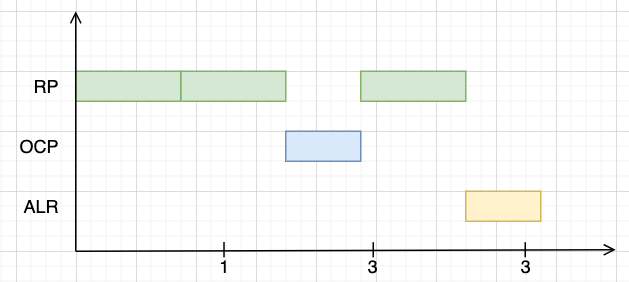
\includegraphics[width=3in]{images/timeline-overload-edf-pattern}
\caption{Timeline of the repeated interval in EDF overloading}
\label{timeline-overload-edf-pattern}
\end{figure}

\section{Conclusions}

We have started off the analysis by seeing the uses of offsets as a mechanism to improve the consistency between a formal model and the runtime execution of a real-time application subject to precedence relations. In turn, this has helped to reduce the pessimism in the fixed-priority analysis and offsets have proved to be extremely useful in increasing the schedulability of a given task set.

Throughout this paper, we have used MAST as model for describing real-time applications and representing not only the characteristics of the architecture of the application but also the hard real-time requirements that are imposed. However, we believe there is still some scheduling theory needed to eliminate some of the restrictions. The combination of all the restrictions has posed a severe blocking issue in our ability to describe a consistent model which could lead to a sound analysis of maximum utilisation. From our experience, the most critical missing pieces are the enhancement of the FPS offset-based analysis between transactions, to make it less pessimist, and the support for EDF offset-based analysis of linear transactions.

Besides, in this paper, we compared the behaviour of the two most famous policies: the FPS and the EDF algorithm. EDF allows a theoretic full processor utilisation, which implies more efficient exploitation of computational resources, but the statement doesn't hold in general with applications composed of dependant tasks.

At the same time, predictability during overload conditions only apply for the highest priority task, and it is not valid in general for the other tasks. Such a property of FPS can be of little use if we do not know a priori which other task is going to overrun \cite{buttazzo-rm-edf}. Under permanent overload conditions, both the behaviours of FPS and EDF are predictable except for an initial interval, but deciding which one is better is highly application conditional. FPS favours high-priority tasks at the expense of the lower ones, whereas EDF exhibits more fairness but provides fewer guarantees on which tasks will meet their deadlines. Nevertheless, what we have presented in this paper is just a shallow insight. Further work is undoubtedly needed to explore better the implications of relation dependencies in FPS and EDF overload.

In this paper, we have also introduced the Deadline-Floor Protocol for controlling access to shared resources within the EDF scheduling framework. This protocol has already been proved to be equivalent to the Stack Resource Protocol, the defacto protocol to use with EDF, by A. Burns (2005) \cite{resource-sharing}. We have instead shown that the combination EDF+DFP can exhibit the same schedule and blocking times of FPS+IPCP in a system where job releases are not stand-alone but instead form a chain.

Therefore, as shown by the aforementioned cases, we believe that the implications of precedence constraints are worth to be the subject of further research.

\bibliographystyle{unsrt}
%\bibliography{references}  %%% Remove comment to use the external .bib file (using bibtex).
%%% and comment out the ``thebibliography'' section.


%%% Comment out this section when you \bibliography{references} is enabled.
\begin{thebibliography}{1}

\bibitem{ycs}
A Burns, B Dobbing, T Vardanega.
\newblock "Guide for the use of the Ada Ravenscar Profile in high integrity systems".
\newblock In {\em University of York Technical Report YCS-2003-348}. January 2003.

\bibitem{arm}
J. Yiu.
\newblock "Exceptions and Interrupts".
\newblock In {\em The Definitive Guide to ARM Cortex-M3 and Cortex-M4 Processors}. October 2013.

\bibitem{ork}
Juan A. de la Puente, José F. Ruiz, Juan Zamorano.
\newblock "Open Ravenscar Real-Time Kernel. Design Definition File, Software Design Document".
\newblock 2001.

\bibitem{mast}
M. Gonzalez Harbour, J.J. GutiCrrez Garcia, J.C. Palencia GutiCrrez, and J.M. Drake Moyano.
\newblock "MAST Modeling and Analysis Suite for Real Time Applications".
\newblock In {\em Proceedings 13th Euromicro Conference on Real-Time Systems}. 2001.

\bibitem{ada-pcp}
Albert M. K. Cheng, James Ras.
\newblock "The Implementation of the Priority Ceiling Protocol in Ada-2005".
\newblock In {\em ACM SIGAda Ada Letters}. Volume XXVII Issue 1, pp 24-39. 2007.

\bibitem{mast-description}
J. M. Drake, M. G. Harbour, J. J. Gutiérrez, P. L. Martínez, J. L. Medina, J. C. Palencia
\newblock "Description of the MAST Model".
\newblock \url{https://mast.unican.es/mast_description.pdf}

\bibitem{mast-analysis}
J. M. Drake, M. G. Harbour, J. J. Gutiérrez, P. L. Martínez, J. L. Medina, J. C. Palencia
\newblock "MAST Analysis Techniques".
\newblock \url{https://mast.unican.es/mast_analysis_techniques.pdf}

\bibitem{mast-restrictions}
J. M. Drake, M. G. Harbour, J. J. Gutiérrez, P. L. Martínez, J. L. Medina, J. C. Palencia
\newblock "MAST Restrictions".
\newblock \url{https://mast.unican.es/mast_restrictions.pdf}

\bibitem{overrundetection}
Juan Zamorano, Alejandro Alonso, José Antonio Pulido, Juan Antonio de la Puente.
\newblock "Implementing Execution-Time Clocks for the Ada Ravenscar Profile".
\newblock In {\em Reliable Software Technologies - Ada-Europe 2004}. pp 132-143. Ada-Europe 2004.

\bibitem{absolute-delay}
Juan Zamorano, Jose F. Ruiz, Juan Antonio de la Puente.
\newblock "Implementing Ada.Real Time.Clock and Absolute Delays in Real-Time Kernels".
\newblock In {\em Reliable SoftwareTechnologies — Ada-Europe 2001}. pp 317-327. Ada-Europe 2004.

\bibitem{rm-dm}
Jane W. S. W. Liu.
\newblock "Rate-Monotonic and Deadline-Monotonic Algorithms".
\newblock In {\em Real-Time Systems}. pp 118-119. 2001.

\bibitem{critical-instants}
Jane W. S. W. Liu.
\newblock "Critical Instants".
\newblock In {\em Real-Time Systems}. pp 131-134. 2001.

\bibitem{optimality-rm-dm}
Jane W. S. W. Liu.
\newblock "Optimality of the RM and DM algorithms".
\newblock In {\em Real-Time Systems}. pp 118-119. 2001.

\bibitem{pcp-blocking}
Jane W. S. W. Liu.
\newblock "Basic Priority Ceiling Protocol - Duration of Blocking".
\newblock In {\em Real-Time Systems}. pp 295-296. 2001.

\bibitem{limited-priorities}
Jane W. S. W. Liu.
\newblock "Limited-Priority Levels".
\newblock In {\em Real-Time Systems}. pp 166-168. 2001.

\bibitem{tick-scheduling}
Jane W. S. W. Liu.
\newblock "Tick Scheduling".
\newblock In {\em Real-Time Systems}. pp 168-171. 2001.

\bibitem{anomalies-multiprocessor}
Jane W. S. W. Liu.
\newblock "Anomalous Behavior of Priority-Driven Systems".
\newblock In {\em Real-Time Systems}. pp 72-73. 2001.

\bibitem{hierarchical-scheduling}
Jane W. S. W. Liu.
\newblock "Schedulability Test of Hierarchically Scheduled Periodic Tasks".
\newblock In {\em Real-Time Systems}. pp 177-179. 2001.

\bibitem{fps-vs-edf}
Jane W. S. W. Liu.
\newblock "Fixed-Priority versus Dynamic-Priority Algorithms".
\newblock In {\em Real-Time Systems}. pp 117-124. 2001.

\bibitem{debug-trace}
Joseph Yiu.
\newblock "Introduction to the Debug and Trace Features".
\newblock In {\em The Definitive Guide to ARM CORTEX-M3 and CORTEX-M4 Processors}. Chapter 4 pp 443-485. 2014.

\bibitem{semihosting}
Joseph Yiu.
\newblock "Semi-hosting".
\newblock In {\em The Definitive Guide to ARM CORTEX-M3 and CORTEX-M4 Processors}. Chapter 18.3 pp 591-595. 2014.

\bibitem{pendsv}
Joseph Yiu.
\newblock "PendSV exception".
\newblock In {\em The Definitive Guide to ARM CORTEX-M3 and CORTEX-M4 Processors}. Chapter 18.3 pp 591-595. 2014.

\bibitem{tindell-dm}
K. Tindell.
\newblock "An Extendible Approach for Analysing Fixed Priority Hard Real-Time Tasks".
\newblock In {\em Journal of Real-Time Systems}. Vol. 6, No. 2, March 1994.

\bibitem{holistic-analysis}
KenTindell, JohnClark.
\newblock "Holistic schedulability analysis for distributed hard real-time systems".
\newblock In {\em Microprocessing and Microprogramming}. Volume 40, Issues 2–3, pp 117-134. April 1994.

\bibitem{liu-utilisation-bound}
C. L. Liu, James W. Layland.
\newblock "Scheduling Algorithms for Multiprogramming in a Hard-Real-Time Environment".
\newblock In {\em Journal of the ACM}. Volume 20 Issue 1, pp 46-61. Jan. 1973.

\bibitem{practitioner}
Klein, M., Ralya, Th., Pollak, B., Obenza, R., Harbour, M.G. .
\newblock "A Practitioner's Handbook for Real-Time Analysis". 1993.

\bibitem{practitioner-utilisation-bound}
Klein, M., Ralya, Th., Pollak, B., Obenza, R., Harbour, M.G. .
\newblock "Using Utilization Bounds for Each Event when Deadlines Are Within the Period".
\newblock In {\em A Practitioner's Handbook for Real-Time Analysis
}. chapter 4.1.2. 1993.

\bibitem{practitioner-growth}
Klein, M., Ralya, Th., Pollak, B., Obenza, R., Harbour, M.G. .
\newblock "Calculating Growth by Increasing Resource Usage of All Events".
\newblock In {\em A Practitioner's Handbook for Real-Time Analysis
}. chapter 4.3.8. 1993.

\bibitem{practitioner-common-data}
Klein, M., Ralya, Th., Pollak, B., Obenza, R., Harbour, M.G. .
\newblock "Designing Tasks that Must Synchronize to Share Common Data".
\newblock In {\em A Practitioner's Handbook for Real-Time Analysis
}. chapter 5.2. 1993.

\bibitem{effects-runtime}
Klein, M., Ralya, Th., Pollak, B., Obenza, R., Harbour, M.G. .
\newblock "Effects of Operating System and Runtime Services on Timing Analysis".
\newblock In {\em A Practitioner's Handbook for Real-Time Analysis
}. chapter 7. 1993.

\bibitem{interrupt-handler}
Klein, M., Ralya, Th., Pollak, B., Obenza, R., Harbour, M.G. .
\newblock "Service the Event at a Specified Software Priority".
\newblock In {\em A Practitioner's Handbook for Real-Time Analysis
}. chapter 5.3.5.2. 1993.

\bibitem{ada-tasks}
Alan Burns, Andy Wellings.
\newblock "Scheduling real-time systems - Fixed Priority Dispatching".
\newblock In {\em Concurrent and real-time programming in Ada}. chapter 13.1. 2007.

\bibitem{timing-events}
Alan Burns, Andy Wellings.
\newblock "Timing events".
\newblock In {\em Concurrent and real-time programming in Ada}. chapter 15.2. 2007.

\bibitem{timing-properties}
Enrico Mezzetti, Marco Panunzio, Tullio Vardanega.
\newblock "Preservation of Timing Properties with the Ada Ravenscar Profile".
\newblock In {\em Reliable Software Technologiey – Ada-Europe 2010}. pp 153-166. 2010.

\bibitem{etc}
Kristoffer Nyborg Gregertsen, Amund Skavhaug.
\newblock "Implementation and Usage of the new Ada 2012 Execution Time Control Features".
\newblock In {\em Ada User Journal}. 2011.

\bibitem{pessimistic-rma}
J.C. Palencia ; M. Gonzalez Harbour.
\newblock "Schedulability analysis for tasks with static and dynamic offsets".
\newblock In {\em Proceedings 19th IEEE Real-Time Systems Symposium}. 1998.

\bibitem{tindell-offsets}
K. Tindell.
\newblock "Adding Time - Offsets to Schedulability Analysis".
\newblock Technical Report YCS 221, Dept. of Computer Science, University of York, England, January 1994.

\bibitem{wcet-problem}
R. Wilhelm et al..
\newblock "The worst-case execution-time problem—overview of methods and survey of tools".
\newblock In {\em Trans. on Embedded Computing Sys}. vol. 7, no. 3, pp. 153, 2008.

\bibitem{spuri}
M. Spuri.
\newblock "Analysis of Deadline Scheduled Real-Time Systems".
\newblock In {\em [Research Report] RR-2772, INRIA}. 1996.

\bibitem{liu-overload}
M. K. Gardner, J. W.S. Liu.
\newblock "Performance of Algorithms for Scheduling Real-Time Systems with Overrun and Overload".
\newblock In {\em Proceedings of 11th Euromicro Conference on Real-Time Systems. Euromicro RTS'99}. 9-11 June 1999.

\bibitem{carletto-edf}
P. Carletto, T. Vardanega.
\newblock "Ravenscar-EDF: Comparative Benchmarking of an EDF Variant of a Ravenscar Runtime".
\newblock In {\em Ada-Europe 2017: Reliable Software Technologies – Ada-Europe 2017}. pp 18-33. 2017.

\bibitem{resource-sharing}
A. Burns.
\newblock "A Deadline-Floor Inheritance Protocol for EDF Scheduled Embedded Real-Time Systems with Resource Sharing"
\newblock Technical Report YCS-2012-476, Department of Computer Science, University of York, UK.

\bibitem{buttazzo-rm-edf}
G.C. Buttazzo.
\newblock "Rate Monotonic vs. EDF: Judgment Day".
\newblock In {\em Real-Time Systems, 2005 - Springer}. 2005.

\bibitem{cervin}
A. Cervin, J. Eker, B. Bernhardsson, K.E. Arzén.
\newblock "Feedback-Feedforward Scheduling of Control Tasks".
\newblock In {\em Real-Time Systems, 2002 - Springer}. 2002.

\bibitem{value-deadline}
G. Buttazzo, M. Spuri, F. Sensini .
\newblock "Value vs. Deadline Scheduling in Overload Conditions".
\newblock In {\em Real-Time Systems, 2002 - Springer}. 2002.

\end{thebibliography}


\end{document}
